% Preamble {{{
\documentclass[12pt]{report}
\usepackage[margin=1in]{geometry}
\geometry{
left=1.2in
}
\usepackage[
backend=biber,
style=numeric,
sorting=none
]{biblatex}
\addbibresource{citations.bib}
\usepackage{graphicx}
\usepackage{float}
\usepackage{array}
\usepackage{caption}
\usepackage{amsmath}
\usepackage{ragged2e}
\usepackage{listings}
\usepackage{titlesec}
\usepackage{hyperref}
\hypersetup{
    colorlinks=true,
		citecolor=black,
    linkcolor=black,
    filecolor=magenta,      
    urlcolor=cyan,
    pdfpagemode=FullScreen,
    }

\lstset{
basicstyle=\small\ttfamily,
columns=flexible,
breaklines=true
}

% Chapter title formatting
\titleformat{\chapter}[display]
  {\normalfont\huge\bfseries\centering}{\centering\chaptertitlename\ \thechapter}{20pt}{\Huge}
\titlespacing*{\chapter} 
  {0pt}{50pt}{40pt}

% Recompile these documents. Do this if you're currently making changes to title and introcution chapters
\includeonly{
	chapters/title,
	chapters/introduction,
}
% }}}

\begin{document}

% Title page %N{{{
\thispagestyle{empty}
\begin{center}
\begin{minipage}{0.75\linewidth}
    \centering

%Thesis title
    {\uppercase{\Large \textbf{Emotion Based Content 
				Discovery System}
\par}}

    \vspace{1cm}
		{Project Report\par}
		{Submitted in partial fulfillment of the requirements\par}
		{For the degree of\par}
		{\textbf{Bachelor of Engineering in Computer Engineering}\par}
    \vspace{1cm}
%Author's name
		{by \par}
		{\Large Neil Botelho - 227668 \par }
		{\Large Suniti Gaonker - 227681 \par}
		{\Large Vivek Silimkhan - 227727 \par}
		{\Large Vipul Chodankar - 227736 \par}
    \vspace{1.5cm}

%Guide
		{\Large Guide - Prof. Maruska Mascarenhas\par}

		\vspace{1.5cm}
%University logo
    
\includegraphics[width=0.3\linewidth]{gecLogo.png}
		\par

%University Name
		\vspace{1.5cm}
		{\LARGE \textbf{Department of Computer Engineering} \par}
			{\LARGE \textbf{Goa College of Engineering} \par}

%Date
		\vspace{2cm}
    {\Large 2022}
\end{minipage}
\end{center}
\clearpage
%}}}


%DO NOT MESS AROUND WITH THE CODE ON THIS PAGE UNLESS YOU %REALLY KNOW WHAT YOU ARE DOING
\begin{center}
%\input{border.sty}
\underline{\bfseries \huge PROJECT APPROVAL SHEET}\\
\vspace{1cm}
\end{center}
\noindent This is to certify that \textbf{Shri Neil Botelho} (bearing Seat no. 227668), \textbf{Shrimati Suniti Gaonker} (bearing Seat no. 227681), \textbf{Shri Vivek Silimkhan} (bearing Seat no. 227727) and \textbf{Shri Vipul Chodankar} (bearing Seat no. 227736) has been admitted to semester VII to the candidacy of degree (Bachelor of Engineering in Computer Engineering) in 2021-2022 and he/she has undertaken the dissertation entitled "\textbf{Emotion Based Content Discovery System}" which is approved for the degree of BE (Computer) under Goa University as it is found satisfactory

\vspace{2.8cm}

\begin{table}[H]
	\begin{center}
\begin{tabular}{lcl}
	\noindent ----------------------------------- &\hspace{1cm}&  ----------------------------------- \\
(Project Guide) & \hspace{3cm} & (Head of Department) \\
Maruska Mascarenhas & \hspace{3cm} & Dr. Jayapura A. Laxminarayana  \\
Associate Professor, Computer Dept. & \hspace{3cm} & Professor, Computer Dept. \\
\end{tabular}
\end{center}
\end{table}

\vspace{2.5cm}

\begin{table}[H]
	\begin{center}
\begin{tabular}{lcl}
	\noindent ----------------------------------- &\hspace{5cm}&  ----------------------------------- \\
(Examiner 1) & \hspace{5cm} & (Examiner 2) \\
\\
\noindent ----------------------------------- &\hspace{5cm} &\noindent ----------------------------------- \\
\\
\noindent ----------------------------------- &\hspace{5cm} &\noindent ----------------------------------- \\

\end{tabular}
\end{center}
\end{table}

\vspace{2cm}

\noindent Date: \\
\\
\noindent Place: \\

% \noindent Place: Farmagudi, Ponda, Goa\\
% \noindent Date: 


\clearpage


\center{\Large{\textbf{Abstract}}\\}
	\vspace{2cm}
	\justifying\small{In the age of streaming and on-demand media, there is an overabundance of content for users to consume. Hence discoverability of new media that is interesting to a user is a massive issue. The current solution is to use opaque algorithms to predict what the user may like. In this project we propose developing a more transparent alternative. This project aims to provide the user a new transparent method of content discovery based on emotions rather than keywords or genres. The user will be provided a set of sliders, each corresponding to a different emotion. Based on the user’s input via the sliders, we they will be recommended songs and movies that match using the system described in this project. } \cite{bert}
\clearpage
\tableofcontents
\listoffigures


\chapter{Introduction}
\section{Overview}
\subsection{Big data in media}
Media and entertainment has become an integrated part of the lives of people, meaning that people nowadays are very enthusiastic about trying new content in terms of watching it and choosing it. Gone are the single-channel days of no choice and no integration and consultation to viewers. But now these dynamics are changing, there are millions of watching options to choose from and they are also available to be streamed across various devices and are really getting user friendly.\newline

Publishers, broadcasters, news organizations, cable companies, and gaming companies in the media and entertainment industry are facing new business models for the way they create, market, and distribute their content. This is happening because today’s consumers search and access content anywhere, at any time, and on any device. As a result, there’s increased pressure to execute new digital production and multi-channel advertising and distribution strategies that rely on a detailed understanding of consumers’ media consumption preferences and behaviors. And, as consumer interests shift from analog to digital media, there are substantial opportunities to monetize content and to identify new products and services. With thousands or millions of digital consumers, media and entertainment companies are in a unique position to leverage their big data assets for more profitable customer engagement. \newline

The scope of big data collected by the media and entertainment industry and the potential to mine it to understand what content, shows, movies, and music consumers want is huge. Viewing history, searches, reviews, ratings, location and device data, clickstreams, log files, and social media sentiment are just a few data sources that help take the guesswork out of identifying audience interest. Using insights from big data, media and entertainment companies are able to understand when customers are most likely to view content and what device they’ll be using when they view it. With big data’s scalability, this information can be analyzed at a granular ZIP code level for localized distribution.

\subsection{AI in media industry}
The media and entertainment industry is also utilizing the power of Artificial Intelligence (AI) in making the visual content more interactive and interesting. It is helping to serve the audience a data-intensive and personalize automated content making their viewing experience more interesting and entertaining.

From music apps to OTT platforms, the audio, as well as visual contents, can be personalized as per the preferences and previous experiences of the user. Using machine learning, users behaviour and demographic details are taken into consideration to provide optimal suggestions for music or videos that they are likely to enjoy.

\subsection{Netflix test case}
Although netflix began as a meagre DVD rental service in 1998 it is now one of the world’s most powerful and renowned media streaming services. Having garnered subscribers up to almost 158.3 million, an estimate of nearly 37\% of the world’s internet users are using Netflix. A large portion of Netflix's growth can be attributed to its  personalized recommendation engine that enables users to find suggestion for new content, personalized to them.  Netflix's personalized recommendation engine is estimated to be worth  1 billion a year and surprisingly 80\% of users stream content suggested by it.

\subsection{Use of Data Science and algorithms to improve customer experience}
In the early 2000s, Netflix had initiated an open competition offering 1 million dollars prize for the best collective filtering algorithm to predict the ratings of users for films, based on their previous ratings. This approach resulted in becoming the turning point for the service.
Now, Netflix uses an opulence of technological algorithms to boost and enhance its customer experience.
In a service like Netflix, every action the user takes is recorded. The shows watched, the time of day when they are viewed, what was watched before and after that show, how quickly a series is binge-watched, when and where a user gets bored and stops watching, how long does a user take to scroll and every single click of the pause and play button. Using a detailed tagging system Netflix is able to recommend it’s users the content which it knows will be their cup of tea.
Recommendation Systems are mainly of two main types :
Content-based Recommendation Systems: In this system, the background knowledge regarding the products as well as the customer information is taken into account. Similar suggestions are provided based on the content the user has viewed on Netflix. For example, if the user has watched a film that has a "thriller" genre, similar films, having the same genre will be suggested.
Collaborative filtering Recommendation Systems: This system provides suggestions based on the similar profiles of its users and is independent of knowledge of the product. This system is based solely on the assumption that what the users prefer in the past they will also prefer in the future.

\section{Motivation}
The outbreak of the Coronavirus (COVID-19) pandemic and its preventative social distancing measures have led to a dramatic increase in subscriptions to paid streaming services. Online users are increasingly accessing live broadcasts, as well as recorded video content and digital music services through internet and mobile devices. In this context, this study aims to explore the individuals’ uses and gratifications from online streaming technologies during COVID-19.
Individuals are increasingly consuming the broadcast media through digital and mobile technologies. Very often, they are watching TV channels, movies, series, shows, etc. through online streaming services that are readily available through ubiquitous technologies, including smartphones or tablets. 
eMarketer (2019) reported that 70.1\% surfed the internet while watching their favorite movies and shows. Moreover, according to the latest Global Web Index Trend Report, the individuals who were between 16–24 years, spent around 7h per day online or on their smartphones or tablets. The individuals from this demographic segment devoted over 2.5 h a day to social networking and were watching more than an hour of online TV per day.\newline

The individuals hailing from the 25–34 age segment have switched from linear TV to online streaming to watch live TV and/or recorded videos. They subscribed to online services through
digital and high-speed mobile devices, including smartphones and tablets to stream live channels and recorded video content from anywhere, at any time (eMarketer, 2019; GWI, 2019). Evidently, they were accessing online streaming through virtual private networks to watch TV programs, movies, entertainment, sporting events and the like (GWI, 2019). Hence, media and entertainment businesses are continuously investing on the programming of new content, including those produced in-house to satisfy their online subscribers. In this light, this study explores the individuals’ perceptions toward online streaming technologies and their motivations to use them to watch recorded videos and/or live broadcasts.\newline

In the age of streaming and on-demand media, there is an overabundance of content for users to consume.
According to FX Networks, in 2019 approximately 532 new scripted tv shows were published.
Spotify reports that over 60,000 new songs are uploaded to its service every day.
Hence discoverability of new media that is interesting to a user is a massive issue. \newline

The current solution is to use opaque algorithms to predict what the user may like. In this project we propose developing a more transparent alternative. 
Due to the addition of a large amount of media everyday, it is the need of hour to make content discovery easy and transparent for the users. 



\chapter{Literature Review}
\section{Genre detection in songs}
Nanni et al. (2018)\cite{nanni_ensemble_2018} investigated the effectiveness of acoustic features versus visual features in music genre detection in their paper Musical genre classification of audio signals. They observed that the features attained by classical methods and the features used by CNN contain different information. By combining the features obtained, they acquired more successful results than previous studies.

Ceylan et al. (2021)\cite{ceylan_automatic_2021} investigated the use of MFCC graphs in music genre detection in their paper Ensemble of deep learning, visual and acoustic features for music genre classification. Music segments from the GTZAN dataset of length 3  seconds were converted into MFCC graphs using python’s librosa library and passed as input into a convolutional neural network. They obtained accuracy comparable to or higher than other studies in which many features or more complex and combined deep learning models were used. 

\section{Emotional models}

The emotional models are classified into 2 major classes as can be seen in Figure \ref{fig: emotional models} one model is categorical and the other is dimensional model \cite{emotion_models}

\subsection{Categorical model}
Emotions are recognized with the help of words denoting emotions or class tags.
The categorical model either makes use of six basic emotion classes namely anger, disgust, fear, joy, sadness, and surprise or uses domain-specific expressive classes such as boredom, confusion. There are both significant and unrelated
emotions in this model. Each emotion has a specific set of features that express provoking circumstances or
reactions. Most research in affective computing has concentrated on the aforementioned six basic emotions
 
 
 
\subsection{Dimensional model}
DImensional model denotes effects in a dimensional form. A common set of dimensions link the various emotional states in this model. They are defined in a
two(valence and arousal) or three ( valence, arousal, and power) dimensional space. Each emotion occupies a position in this space. The valence dimension defines the positivity or negativity of emotion and ranges from unpleasant feelings to pleasant feelings (sense of happiness). The arousal dimension denotes the level of excitement that the emotion depicts, and it ranges from sleepiness or boredom to wild excitement. The influence dimension denotes the degree of power such as a sense of control over the emotion.

\begin{figure}[H]
\centering
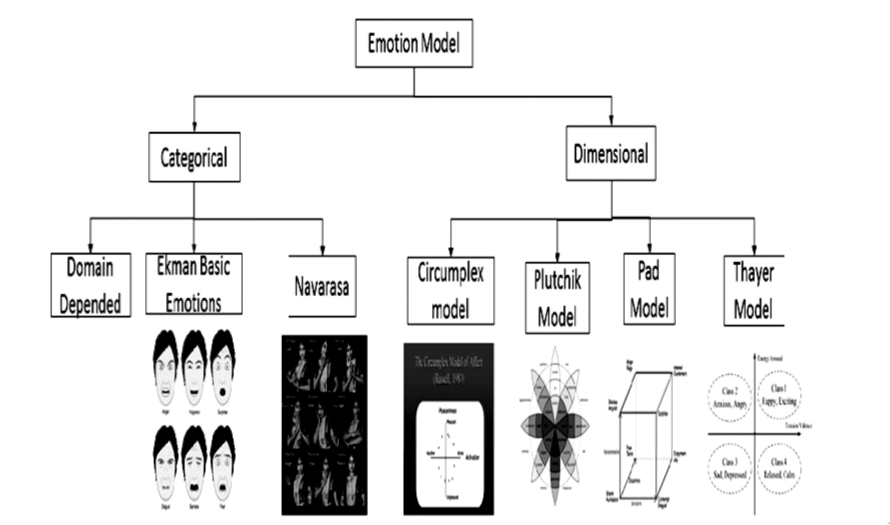
\includegraphics[width=\textwidth]{imgs/emotion_models.png}
\caption{Emotional Models}
\label{fig: emotional models}
\end{figure}

\section{Plutchik emotional model}
Plutchik \cite{plutchik_emotions} states that there are eight basic emotions: 
\begin{enumerate}
	\item Joy
	\item Trust
	\item Fear
	\item Surprise
	\item Sadness
	\item Anticipation
	\item Anger
	\item Disgust
\end{enumerate}
Plutchik created the wheel of emotions as can be seen in Figure \ref{fig: plutchik model}, which illustrates the various relationships among the emotions. \newline

Each primary emotion also has a polar opposite, so that:
\begin{itemize}
	\item Joy is the opposite of sadness.
	\item Fear is the opposite of anger.
	\item Anticipation is the opposite of surprise.
	\item Disgust is the opposite of trust.
\end{itemize}


\begin{figure}[H]
\centering
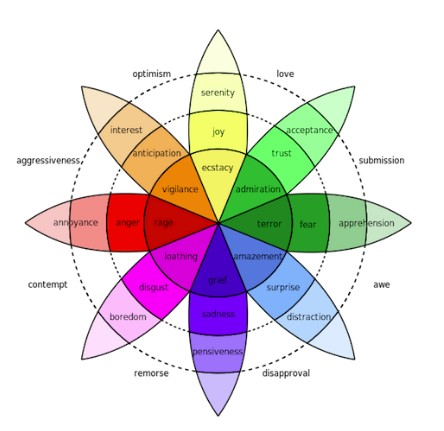
\includegraphics[width=\textwidth]{imgs/plutchik_model.jpg}
\caption{Plutchik's Emotional Model}
\label{fig: plutchik model}
\end{figure}


\section{Web Scraping}
Web scraping, also known as web extraction or harvesting, is a technique to extract data from the World Wide Web and save it to a file system or database for later retrieval or analysis\cite{webscraping}\newline

Web scraping is accomplished either manually by a user or automatically by a bot or web crawler. Due to the fact that an enormous amount of heterogeneous data is constantly generated on the World Wide Web.\newline

To adapt to a variety of scenarios, current web scraping techniques have become customized from smaller ad hoc, human-aided procedures to the utilization of fully automated systems that are able to convert entire websites into well-organized datasets, and are often performed using automated tools.
\section{Mel Scale}
The Mel scale is a fundamental result of psychoacous tics, relating real frequency to perceived frequency. The foundation of the mel scale is the classic work of Stevens and Volkman\cite{mel-scale}. Their results and variations thereof appear in almost every speech book. In this paper we address certain issues regarding the Mel scale and in particlar we discuss the issue of fitting the Mel scale and the implications and physical meaning of the fitting formula. Many authors have attempted fit ting formulas for a variety of reasons. Most important among these is that such fits sometimes give an indi cation of the underlying physical phenomenon. Furthermore, such fits may be used to develop models for the psychoacoustic scale. \newline

An alternate definition of the mel scale is that it is a quasi-logarithmic function of acoustic frequency designed such that perceptually similar pitch intervals (e.g. octaves) appear equal in width over the full hearing range.

\section{MFCC}
Mel Frequency Cepstrum or MFC is a representation of the short-term power spectrum of a sound, which is based on a linear cosine transform of a log power spectrum on a nonlinear mel scale of frequency. A visualization of an MFCC can be seen in Figure \ref{fig: mfcc}
Mel Frequency Cepstrum Coefficients or MFCC are the coefficients that make up the MFC representation  \cite{mel-frequency_2021} \newline

Standard MFCC computation technique utilizes discrete cosine transform (DCT) for decorrelating log energies of filter bank output. The use of DCT is reasonable here as the covariance matrix of Mel filter bank log energy or MFLE can be compared with that of highly correlated Markov-I process.\cite{mfcc_speaker_2012}

\begin{figure}[H]
\centering
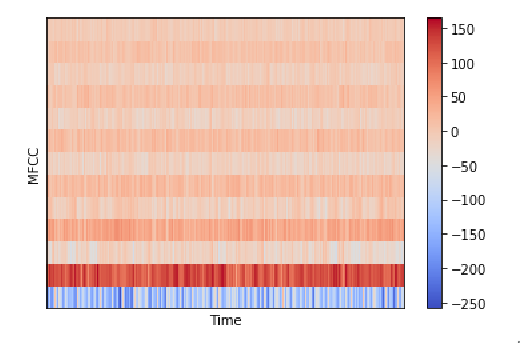
\includegraphics[width=\textwidth]{imgs/mfcc.png}
\caption{MFCC spectrum}
\label{fig: mfcc}
\end{figure}


\section{Existing corpora for emotion classification in text}
Bostan and Klinger (2018) \cite{emotion_classification_datasets}, performed an analysis on existing corpora for emotion classification in text. They analyzed 14 existing emotion datasets, nearly all of which use an annotation scheme based on Ekman (Ekman, 1969 \cite{ekman_pan-cultural_1969}) with many adding a few labels often following Plutchik’s theory of emotions (Plutchik, 1980 \cite{plutchik_emotions})


\section{The GTZAN dataset}
Tzanetakis and Cook (2002)\cite{tzanetakis_musical_2002}  investigated automatically classifying audio signals into a hierarchy of musical genres namely:

\begin{itemize}
	\item Classical
	\item Country
	\item Disco
	\item Hiphop
	\item Jazz
	\item Rock
	\item Blues
	\item Reggae
	\item Pop
	\item Metal
\end{itemize}

These researchers made use of several musical features such as rhythm, timbre, and pitch in the process of classifying music. They also produced the most widely used dataset for music genre detection, the GTZAN dataset \cite{gtzan_dataset}

\section{XED dataset}
The XED dataset was produced by Ohman et. al. \cite{ohman-etal-2020-xed}. The XED dataset uses Plutchik’s core emotions as its annotation scheme resulting in 8 distinct emotion categories plus neutral. The dataset uses the OPUS (Lison and Tiedemann, 2016 \cite{opensubtitles2016}) parallel movie subtitle corpus of subtitles collected from opensubtitles.org \newline

The dataset consists of tab separated files(tsv) mapping lines from the subtitles to emotions from Plutchik’s model.

\section{Convolutional Neural Network}
Convolutional neural networks are distinguished from other neural networks by their superior performance with image, speech, or audio signal inputs. They have three main types of layers, which are:
\begin{itemize}
	\item Convolutional layer
	\item Pooling layer
	\item Fully-connected (FC) layer
\end{itemize}

The convolutional layer is the first layer of a convolutional network. While convolutional layers can be followed by additional convolutional layers or pooling layers, the fully-connected layer is the final layer. With each layer, the CNN increases in its complexity, identifying greater portions of the image. Earlier layers focus on simple features, such as colors and edges. As the image data progresses through the layers of the CNN, it starts to recognize larger elements or shapes of the object until it finally identifies the intended object.\newline

The convolutional layer is the core building block of a CNN, and it is where the majority of computation occurs. An illustration of this computation is shown in Figure \ref{fig: cnn}. It requires a few components, which are input data, a filter, and a feature map. Let’s assume that the input will be a color image, which is made up of a matrix of pixels in 3D. This means that the input will have three dimensions—a height, width, and depth—which correspond to RGB in an image. We also have a feature detector, also known as a kernel or a filter, which will move across the receptive fields of the image, checking if the feature is present. This process is known as a convolution.

\begin{figure}[H]
\centering
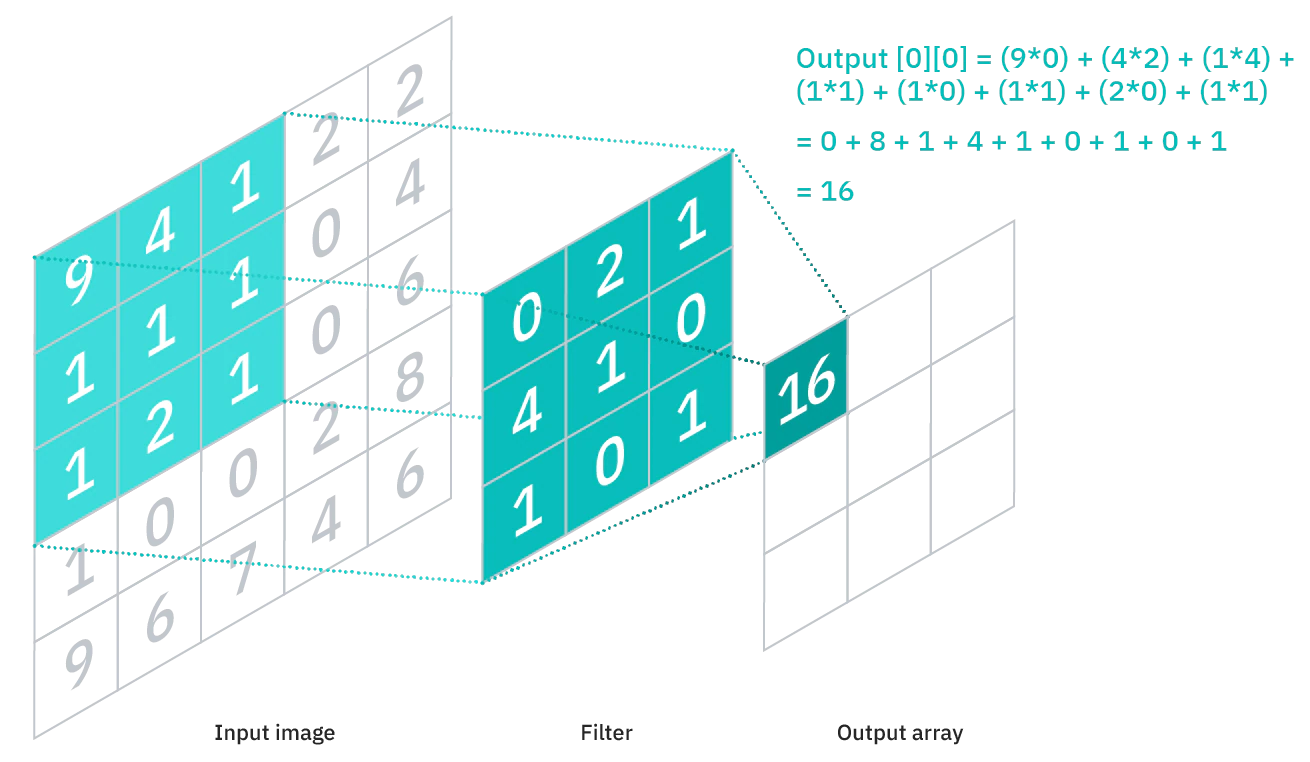
\includegraphics[width=\textwidth]{imgs/cnn.png}
\caption{Working of a Convolutional Neural Network}
\label{fig: cnn}
\end{figure}
\section{Recurrent Neural Network}
A recurrent neural network (RNN) is a type of artificial neural network which uses sequential data or time series data. These deep learning algorithms are commonly used for ordinal or temporal problems, such as language translation, natural language processing (nlp), speech recognition, and image captioning; they are incorporated into popular applications such as Siri, voice search, and Google Translate. Like feedforward and convolutional neural networks (CNNs), recurrent neural networks utilize training data to learn. They are distinguished by their "memory" as they take information from prior inputs to influence the current input and output. While traditional deep neural networks assume that inputs and outputs are independent of each other, the output of recurrent neural networks depend on the prior elements within the sequence as can be seen in Figure \ref{fig: rnn}. While future events would also be helpful in determining the output of a given sequence, unidirectional recurrent neural networks cannot account for these events in their predictions.

\begin{figure}[H]
\centering
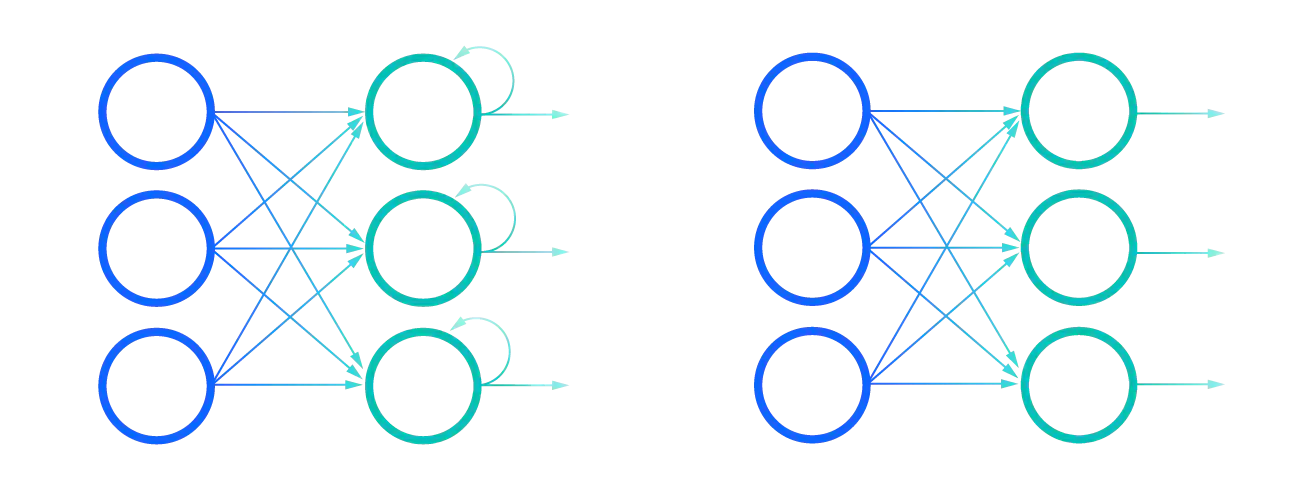
\includegraphics[width=\textwidth]{imgs/rnn.png}
\caption{Recurrent Neural Network vs. Feedforward Neural Network }
\label{fig: rnn}
\end{figure}
\section{Transfer Learning}
The reuse of a pre-trained model on a new problem is known as transfer learning in machine learning \cite{transfer_learning}. A machine uses the knowledge learned from a prior assignment to increase prediction about a new task in transfer learning. The knowledge of an already trained machine learning model is transferred to a different but closely linked problem throughout transfer learning as illustrated in \ref{fig: transferLearning}. For example, if you trained a simple classifier to predict whether an image contains a backpack, you could use the model’s training knowledge to identify other objects such as sunglasses. \newline

In computer vision, neural networks typically aim to detect edges in the first layer, forms in the middle layer, and task-specific features in the latter layers. The early and central layers are employed in transfer learning, and the latter layers are only retrained. It makes use of the labelled data from the task it was trained on.

\begin{figure}[H]
\centering
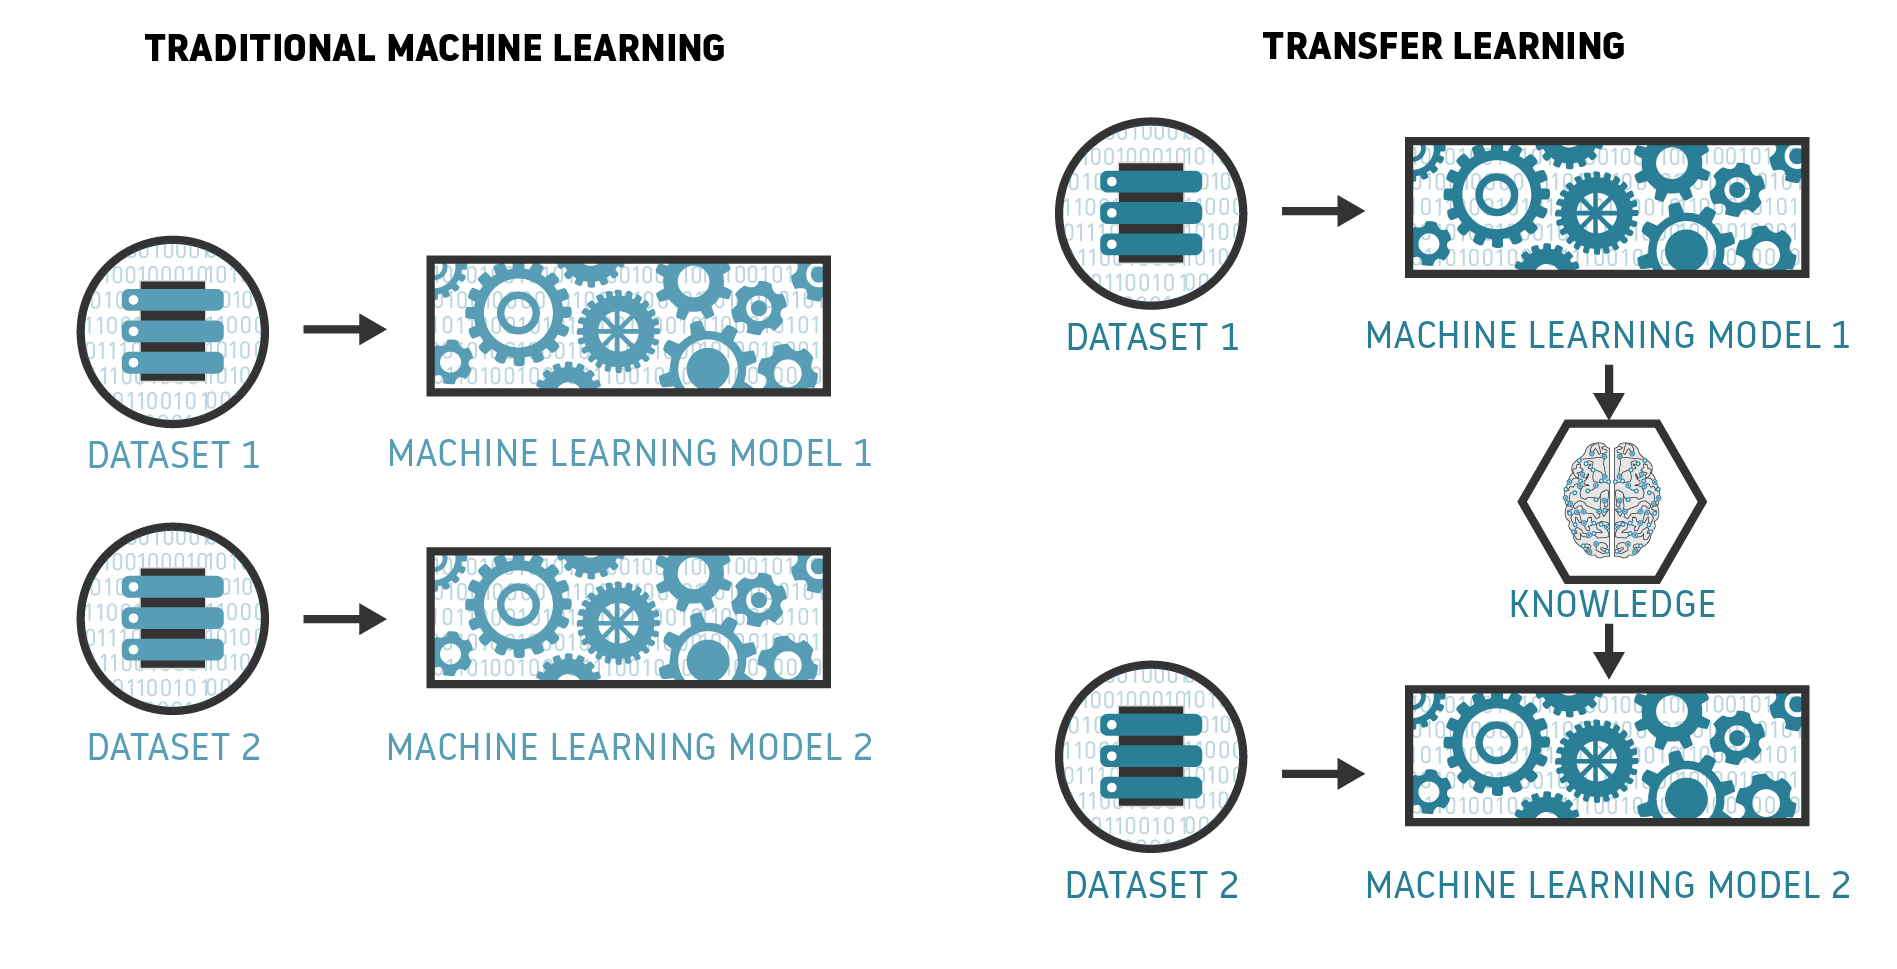
\includegraphics[width=\textwidth]{imgs/transferlearning.jpg}
\caption{Transfer Learning}
\label{fig: transferLearning}
\end{figure}


\chapter{Project Requirements}
\section{Hardware Requirements}
\begin{table}[H]
\normalsize
\begin{center}
\begin{tabular}{|m{2.5cm}| m{7cm}|}
	\hline
	\textbf{Hardware} & \textbf{Specifications}\\
	\hline
	RAM  & 1GB Minimum \\
	\hline
Disk Space & Minimum 2GB storage space\\
	\hline
Connectivity & 2G connection Minimum\\
	\hline
\end{tabular}
\end{center}
\end{table}

\section{Software Requirements}
\begin{table}[H]
\normalsize
\begin{center}
\begin{tabular}{|m{2.5cm}| m{8cm}|}
	\hline
	\textbf{Software} & \textbf{Specifications}\\
	\hline
OS & Windows, Linux, Mac, Android or IOS\\
	\hline
Browser & Google Chrome, Safari, Mozilla Firefox, Opera or Microsoft Edge must be installed\\
	\hline
\end{tabular}
\end{center}
\end{table}

\section{Technologies Used}

\subsection{ReactJS}
ReactJS is a front-end JavaScript library for building reusable User Interface components.  These componentIt provides the View layer in the Model View Controller(MVC) paradigm. It can be used in developing Single Page Applications. React components make it possible to develop large web based applications efficiently. These applications provide better user experience, are interactive and faster because the data can be changed without subsequent page refreshes. 


\subsection{Node.js}
Node.js is an open-source, cross-platform, JavaScript runtime environment. It executes JavaScript code outside of a web browser. It is used by web developers for server side scripting to produce dynamic web page content before sending it to the user. Node.js allows web development around a single programming language by eliminating the need to use programming languages other than JavaScript for backend development. \newline

It has an event-driven architecture that is capable of asynchronous I/O, enabling development of fast web servers in JavasScript. This makes the web application scalable and suitable for real time applications like browser games. Node.js is officially supported on Linux, macOS and Microsoft Windows 8.1.

\subsection{Python}
Python is a high level, general purpose programming language. It supports multiple programming paradigms including functional and object oriented programming. It was designed for code readability. The formatting is visually uncluttered and uses English keywords. It is one of the most popular programming languages. It allows programmers to write clear and logical code for small as well as large scale projects. \newline

Python source distribution maintains "batteries included philosophy" for having a rich and versatile standard library. This gives Python language a head start in many projects since the developer can start working on the project directly, without installing additional packages. 

\subsection{Librosa}
Librosa is a python package for music and audio analysis. It provides the building blocks necessary to create music information retrieval systems. It uses different signal processing techniques for visualization of audio signals as well as for feature extraction. \newline

Librosa is structured as a collection of submodules that contains functions for estimating tempo, detecting beat events, visualization, time-domain audio processing, feature extraction and so on.

\subsection{TensorFlow}
TensorFlow is a free and open source software library for Machine Learning and Artificial Intelligence. It can be used in a wide variety of programming languages like Python, Javascript and so on. Its flexible architecture allows it to be used across variety of platforms \newline

The features of this library includes
\begin{itemize}
	\item AutoDifferentiation : process of automatically calculating the gradient vector of a model with respect to each of its parameters
	\item Eager execution : operations are evaluated immediately as opposed to being added to a computational graph which is executed later
	\item Losses : For training and accessing models
	\item Metrics : API access to commonly used metrics
\end{itemize}
And more.

\subsection{MongoDB}
MongoDB is a document oriented database platform. It is a NoSQL database program and uses JSON-like documents with optional schema. It is schema less, that is the number of fields, content and size of one document can differ from other documents. The structure of single object is clear and there are no complex joins\newline

MongoDB supports dynamic queries that are as powerful as SQL. It is easily scalable. It provides faster data access since it used internal memory for storing the working set. It can be used for applications involving Big Data, Data Hub, Content Management and Delivery, User Data Management, etc.

\subsection{Hyper Text Markup Language (HTML)}
Hypertext refers to the links on the internet. Markup Language is a standardized text-encoding system that is used to control structure and formatting of a text document. HTML is a Hypertext Markup Language that is used as a standard for describing documents on the web. \newline

HTML documents are basic building blocks of the web and they are accessible and interconnected with the help of links. HTML elements are used to build HTML pages. These elements are represented in the form of tags. A tag consists of the element name surrounded by angle brackets "\textless" and "\textgreater". These tags allow document content to be represented in the form of headings, paragraphs, lists, links, images and so on. 

\subsection{Cascading Style Sheets (CSS)}
CSS is a style sheet language used to describe the presentation of a document written in a markup language like HTML. Presentation includes layout, colors, fonts and so on. It describes how elements should be rendered. \newline

CSS makes it possible to separate content from presentation. This allows more flexibility and control to describe presentation characteristics. It also makes it possible to use the same formatting for different documents. Writing CSS separately in a .css file reduces repetitive code and allows it to be cached for faster load speed.  With the help of CSS, the same markup page can be rendered differently.




\chapter{Proposed Work}
\section{Problem Statement}
This project aims to provide the user a new transparent method of content discovery. The user will be provided a set of sliders, each corresponding to a different emotion. Based on the user’s input via the sliders, we will recommend songs and movies that match. \newline

Since most of the content discovery systems provide searches based on the video name or song name a content discovery system based on emotions will help the user find desirable content and also help the user explore content which the user might not have come across.

\section{Objectives}
\begin{itemize}
	\item To classify movies and songs along a set a emotions using subtitles and song content resp.
	\item To automate addition of new movies and songs to the dataset via scraping for subtitles and song audio
	\item To recommend movies and songs according to the kind of media the user wants to watch
	\item To take into account preferences of other similar users when making a recommendation to a user
\end{itemize}
\chapter{Design}
\section{Data Flow Diagram}

\begin{figure}[H]
\centering
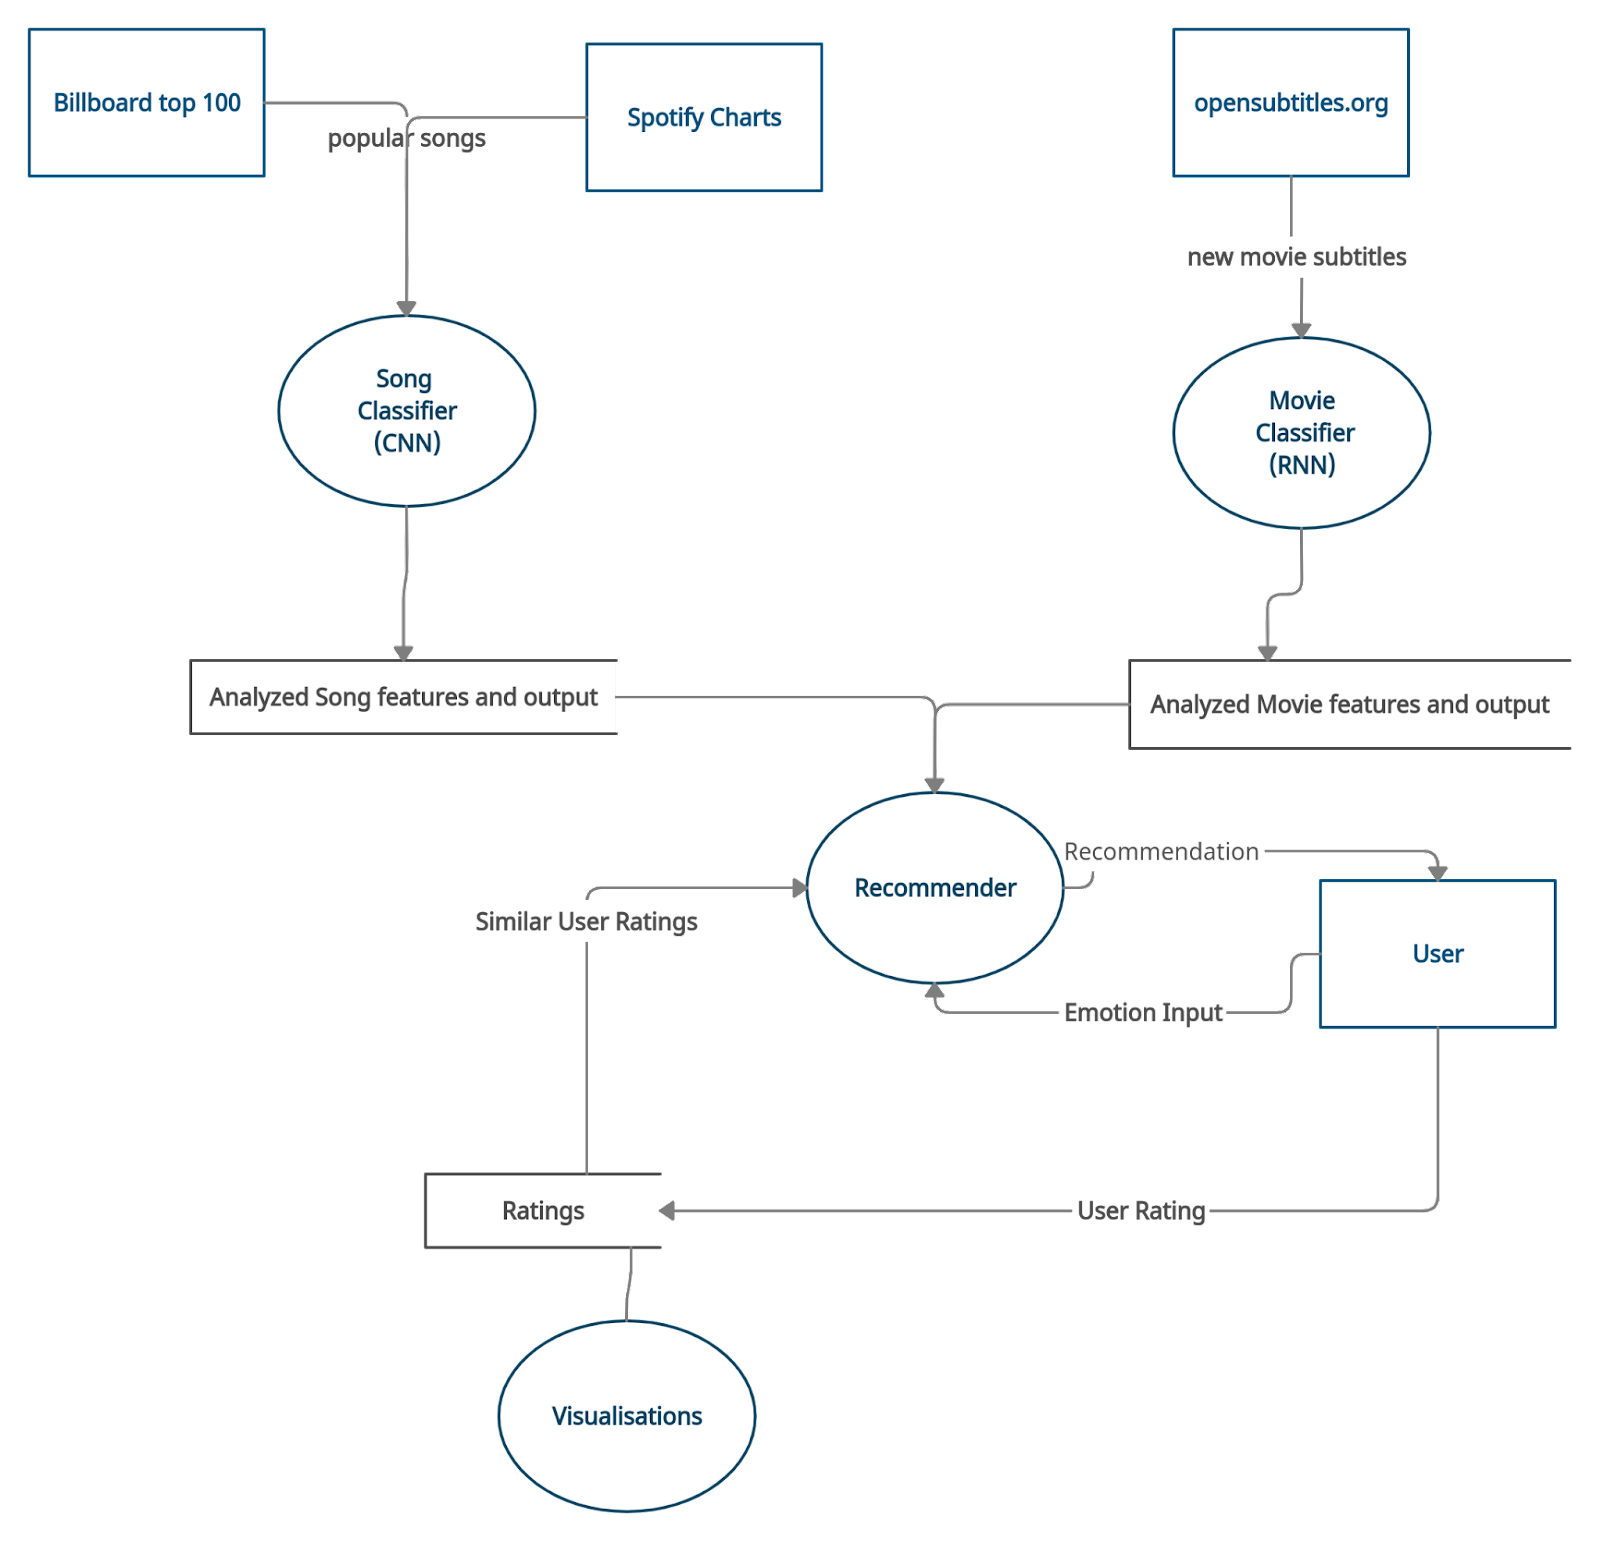
\includegraphics[scale=0.19]{imgs/dataFlowDiagram.png}
\caption{Data Flow Diagram}
\label{fig: data flow diagram}
\end{figure}

\section{ER Diagram}
\begin{figure}[H]
\centering
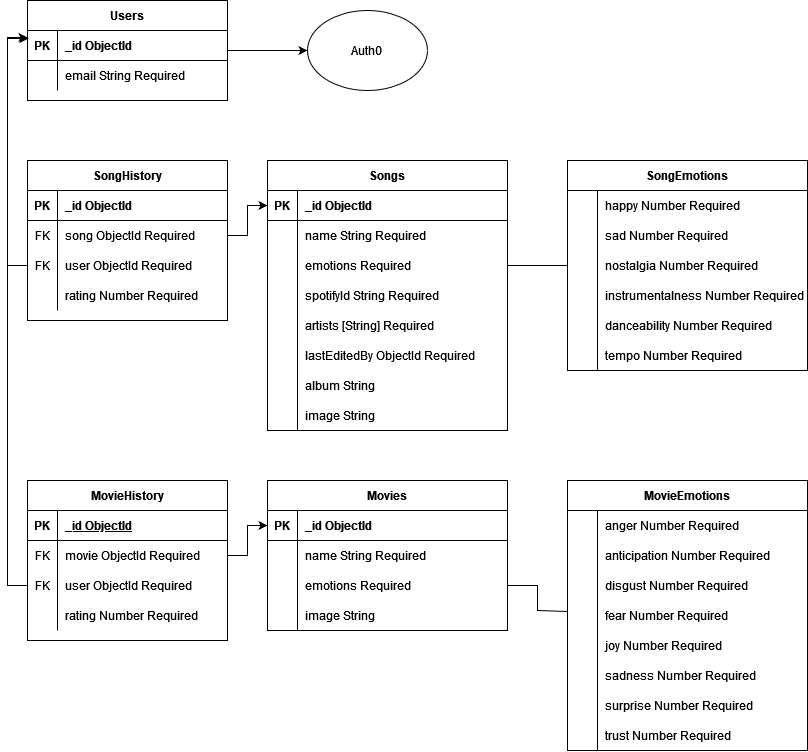
\includegraphics[width=\textwidth]{imgs/erDiagram.png}
\caption{ER Diagram}
\label{fig: erDiagram}
\end{figure}
For our app's class diagram (as shown in Figure \ref{fig: erDiagram} ), we have 5 entities. A unique ObjectId (\_id) attribute is common to all entities. In addition to this, each entity has the following attributes:
\begin{enumerate}

\item Users: The attribute email is of datatype String

\item SongHistory:
	\begin{itemize}
		\item The attributes song and user are of datatype ObjectId,
		\item The attribute rating is of datatype Number.
	\end{itemize}

\item MovieHistory:
	\begin{itemize}
	\item The attributes movie and user are of datatype ObjectId,
	\item The attribute rating is of datatype Number.
	\end{itemize}


\item Songs:
	\begin{itemize}
		\item The attributes name, spotifyId, album and image are of datatype String.
		\item The attribute emotions is an emdedded document containing attributes happy, sad, nostalgia, instrumentalness, danceability and tempo of datatype Number
		\item The attribute artists will be stored in an array of Strings.
	\end{itemize}

\item Movies:
	\begin{itemize}
		\item The attributes name, image are of datatype String.
		\item The attribute emotions is an emdedded document containing attributes anger, anticipation, disgust, fear, joy, sadness, surprise and trust of datatype Number
	\end{itemize}
\end{enumerate}

\section{Use case diagram}
A UML case diagram is the primary form of system/software requirements for a new software program underdeveloped. Use cases specify the expected behavior (what), and not the exact method of making it happen (how). Use cases once specified can be denoted both textual and visual representation (i.e., use case diagram). A key concept of use case modeling is that it helps us design a system from the end user's perspective. It is an effective technique for communicating system behavior in the user's terms by specifying all externally visible system behavior.

The main purpose of a use case diagram is to portray the dynamic aspect of a system. It accumulates the system's requirement , which includes both internal as well as external influences. It invokes persons, use cases and several things that invoke the actors and elements accountable for the implementation of use  case diagrams. It represents how an entity from the external environment can interact with a part of the system.
\begin{figure}[H]
\centering
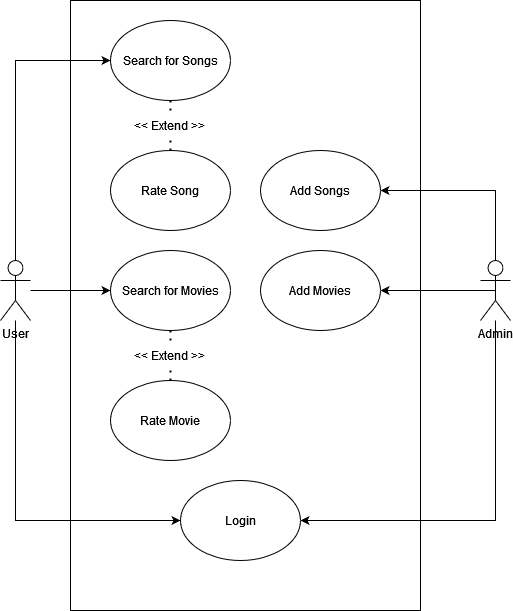
\includegraphics[width=\textwidth]{imgs/use_case.png}
\caption{Use case diagram}
\label{fig: usecase}
\end{figure}


For the use case diagram of our app (shown in Figure \ref{fig: usecase}), there are 2 actors (Someone who interacts with use case/triggers  the use case (system function)) - User and Admin. The ellipses/bubbles represent the system functions/use cases. \newline

The use cases we have for the users are:
\begin{itemize}
\item Search Songs
\item Search Movies
\item Login
\end{itemize}

The use cases we have for the admins are:
\begin{itemize}
\item Add Songs
\item Add Movies
\item Login
\end{itemize}

Extend relationship is used when a use case adds steps to another first-class use case. In our app, the user can choose to rate the song or movie if they are logged in and wish to do so. 


\chapter{Planned Implementation}
\section{Emotion Input}
This will be an interface, that end users use for inputting emotions. It will consist of a slider for each emotion for that particular media(i.e. separate emotions for movies and songs). The value will be a floating point number with a range from 0 to 1. Once the emotions are submitted by the end user, they will be normalized by dividing each emotion by the sum of all emotions. i.e.

 $$ E_{a} = \frac{e_{a}}{\sum_{i=0}^{n}{e_{i}}} $$
\begin{align*}
\text{where } E_{a} &= \text{Normalized value of } e_{a}  \\
e_{i} &= \text{magnitude of emotion } e_{i} \text{ as input by user}\\
n &= \text{number of emotions accepted}
\end{align*}

\section{Authentication}
To be implemented with Auth0, JSON Web Tokens (JWTs) and the modern OAuth 2.0 framework. We will be providing login using various services like Google, Twitter, GitHub etc. This increases security by avoiding the need to have the user remember a secure and complicated password. The aim is to make the authentication process as simple as ‘one click to get started’. This approach also allows us to reuse industry standard components rather than needing to reinvent the wheel. The architecture of OAuth 2.0 is shown in Figure \ref{fig: oAuth uml}

\begin{figure}[H]
\centering
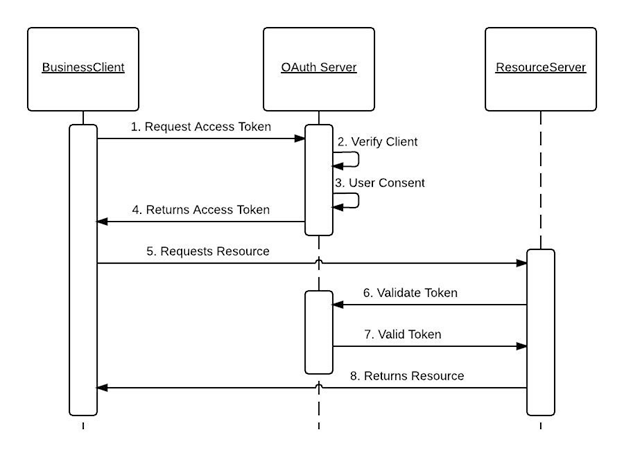
\includegraphics[width=\textwidth]{imgs/oAuth.png}
\caption{OAuth 2.0 Architecture Diagram}
\label{fig: oAuth uml}
\end{figure}
\section{Song Classifier}

\subsection{The Dataset}
2 datasets will be used to train the model, namely:
\begin{enumerate}
	\item The GTZAN dataset
	\item A custom dataset of around 200 songs hand labeled 
\end{enumerate}
The custom dataset will be generated by us using a data collection tool as detailed below.

\subsection{The Model}
The initial architecture of the model to be trained is based on a paper by Ceylan et. al. \cite{ceylan_automatic_2021}. It involves using Mel Frequency Cepstrums(MFC’s) as inputs to a CNN. MFC’s allow us to visualise the different features of a signal at different points of time. \newline

The model will be trained on genre detection using the GTZAN dataset. Once sufficient accuracy is achieved, transfer learning will be used to train the model on the custom dataset to obtain the output we desire. \newline


Two kinds of models will be investigated, namely

\begin{enumerate}
	\item Artificial neural network (ANN)
	\item Convolution neural network (CNN)
\end{enumerate}
The ANN will consist of only dense layers and will take tabular inputs. These inputs will be descriptive features of the input songs like MFCC, spectral centroid, spectral rolloff, chroma frequencies, tempo etc. The CNN will take MFC visualizations and spectrograms as inputs.

\subsection{Model Architecture}

\begin{figure}[H]
\centering
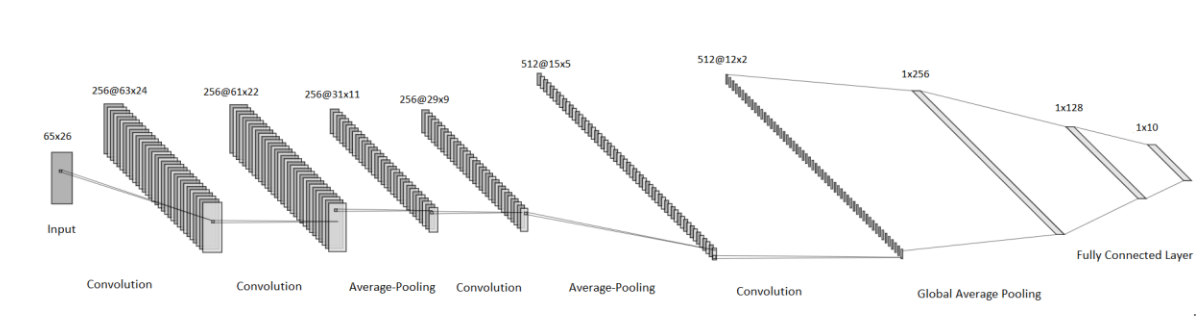
\includegraphics[width=\textwidth]{imgs/model_architecture.png}
\caption{CNN Model Architecture}
\label{fig: cnn architecture}
\end{figure}


The model used in the paper has the following architecture as shown in Figure \ref{fig: cnn architecture}:

\begin{itemize}
	\item Convolution Layer with filters: 256, kernel size: 3x3, 
	\item Convolution Layer with filters: 256, kernel size: 3x3, 
	\item Average Pooling with pool size: 3x3, strides: 2x2, 
	\item Convolution Layer with filters: 256, kernel size: 3x3,
	\item Average Pooling with pool size: 3x3, strides: 2x2, 
	\item Convolution Layer with filters: 512, kernel size: 4x4, 
	\item Global Average Pooling,
	\item Fully Connected Layer,
	\item Dense Layer with units: 256, 
	\item Dense Layer with units: 128, 
	\item Dense Layer with units: 10, activation function: softmax
\end{itemize}

\section{Movie Classifier}
\subsection{The Dataset}
The dataset that will be used to train the model is the XED dataset. This dataset maps movie subtitles to Plutchik's wheel of emotions. Each record in this dataset is an individual sentence mapped to an emotion. \newline

\subsection{The Model}
The model will be a RNN, i.e. it will have one or more recurrent layers like a LSTM or GRU layer. This model will be trained on individual lines from subtitles. To classify a movie, the model will be run on every line of its subtitles. Lines that get classified as neutral are discarded. The sum of the number of lines belonging to each emotion category are then normalized. This gives us a single vector of emotions with values ranging from 0 to 1.
\subsection{Model Architecture}
The initial architecture of the model to be trained will be based on a paper by Hidayatullah et. al. \cite{rnn-sentiment}, where sentiment analysis was used on twitter data to predict the winner of the Indonesian Presidential Election. The model architecture used in the paper is shown in Figure \ref{fig: movieModelArch}


\begin{figure}[H]
\centering
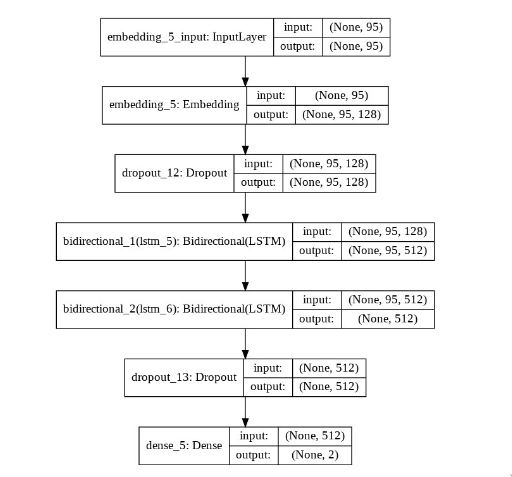
\includegraphics[width=\textwidth]{imgs/movieModelArch.png}
\caption{Sentiment Analysis Model Architecture}
\label{fig: movieModelArch}
\end{figure}
The main change to be made to this model for the purposes of this project is to change the number of neurons in the final layer to the number of emotions we want to predict. 
\section{Media Search \& Recommender System:}
This system will consist of 2 modules i.e. a Media Lookup Module and a Recommender System.

\begin{figure}[H]
\centering
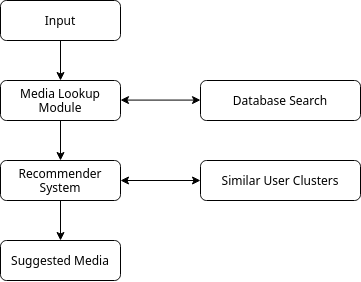
\includegraphics[scale=0.6]{imgs/mediaSearchuml.png}
\caption{Flow for Media Search and Recommender Module}

\label{fig: mediaUML}
\end{figure}
\subsection{Media lookup module}
Based on the user’s inputted emotions, this module will perform a search on the classified songs and movies in the database and return the closest 20 items. To find the best matches, distance measures based on Minkowski distance like Euclidean and Manhattan distance, and also Cosine distance will be tested. The distance measure with the best results will be picked.

\subsection{Recommender System}
Since emotions are subjective, if one movie in the database is slightly closer to the inputted emotion than another movie, it doesn't necessarily mean that the closer movie is better. To address this subjectivity in the inputted emotion, the Media Search module is augmented by a recommendation system that users similar users preferences to decide which movies/songs should be ranked higher, i.e. which movies/songs are better matches for that particular user. \newline

As the user views the songs/movies, if he/she rates them, that rating is stored and used for future recommendations. Once the user has some minimum threshold number of ratings, we can augment the simple search with a recommendation system.

\subsubsection{Prerequisites}
\begin{enumerate}
	\item A matrix of user-movie ratings as shown in Figure \ref{fig: user movie ratings} will be maintained
	\item Users should periodically be clustered based on their movie ratings using KNN algorithm
\end{enumerate}

\begin{figure}[H]
\centering
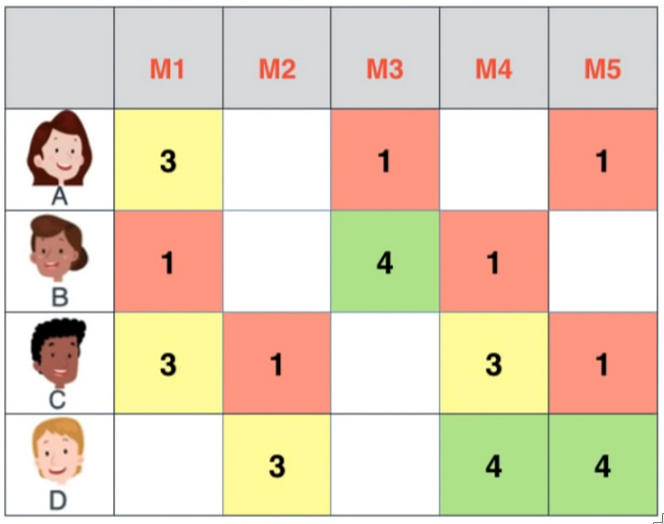
\includegraphics[scale=0.5]{imgs/user-movie ratings.png}
\caption{User-Movie ratings matrix}
\label{fig: user movie ratings}
\end{figure}

\subsubsection{Recommendation Algorithm}
To recommend new movies to a particular user A:
\begin{enumerate}
	\item Consider the ratings of all other users in the same cluster
	\item Take a weighted average of all movies user A hasn’t seen. Let the weight be the inverse of distance of that user from user A
	\item Recommend the movies with highest score to user A
\end{enumerate}

To illustrate we have also included the formula here below :
$$ Score = \frac{\sum_{i=0}^{m}{\frac{R_{i}}{d_{i}}}}{n}      $$

\begin{align*}
\text{where } R_{i} &= \text{Ratings by user} i  \\
d_{i} &= \text{distance between user } A \text{and user }i\\
n &= \text{number of users in cluster} \\
m &= \text{number of movies in matrix}
\end{align*}

\section{Data Collection Tool}
The capabilities of this tool is as follows:
\begin{itemize}
	\item A tool that connects to Spotify and allows the user to search for and label songs.
	\item Search for a song, listen to it and label it from just one location.
	\item Designed for mobile usage as well, so it can be used on the go too.
\end{itemize}

This tool is built into our application as an admin dashboard. It utilizes Spotify’s API which is free for non-commercial usage to fetch song data. It is connected to MongoDB via Node.js APIs.
\subsection{Desktop View}
\begin{figure}[H]
\centering
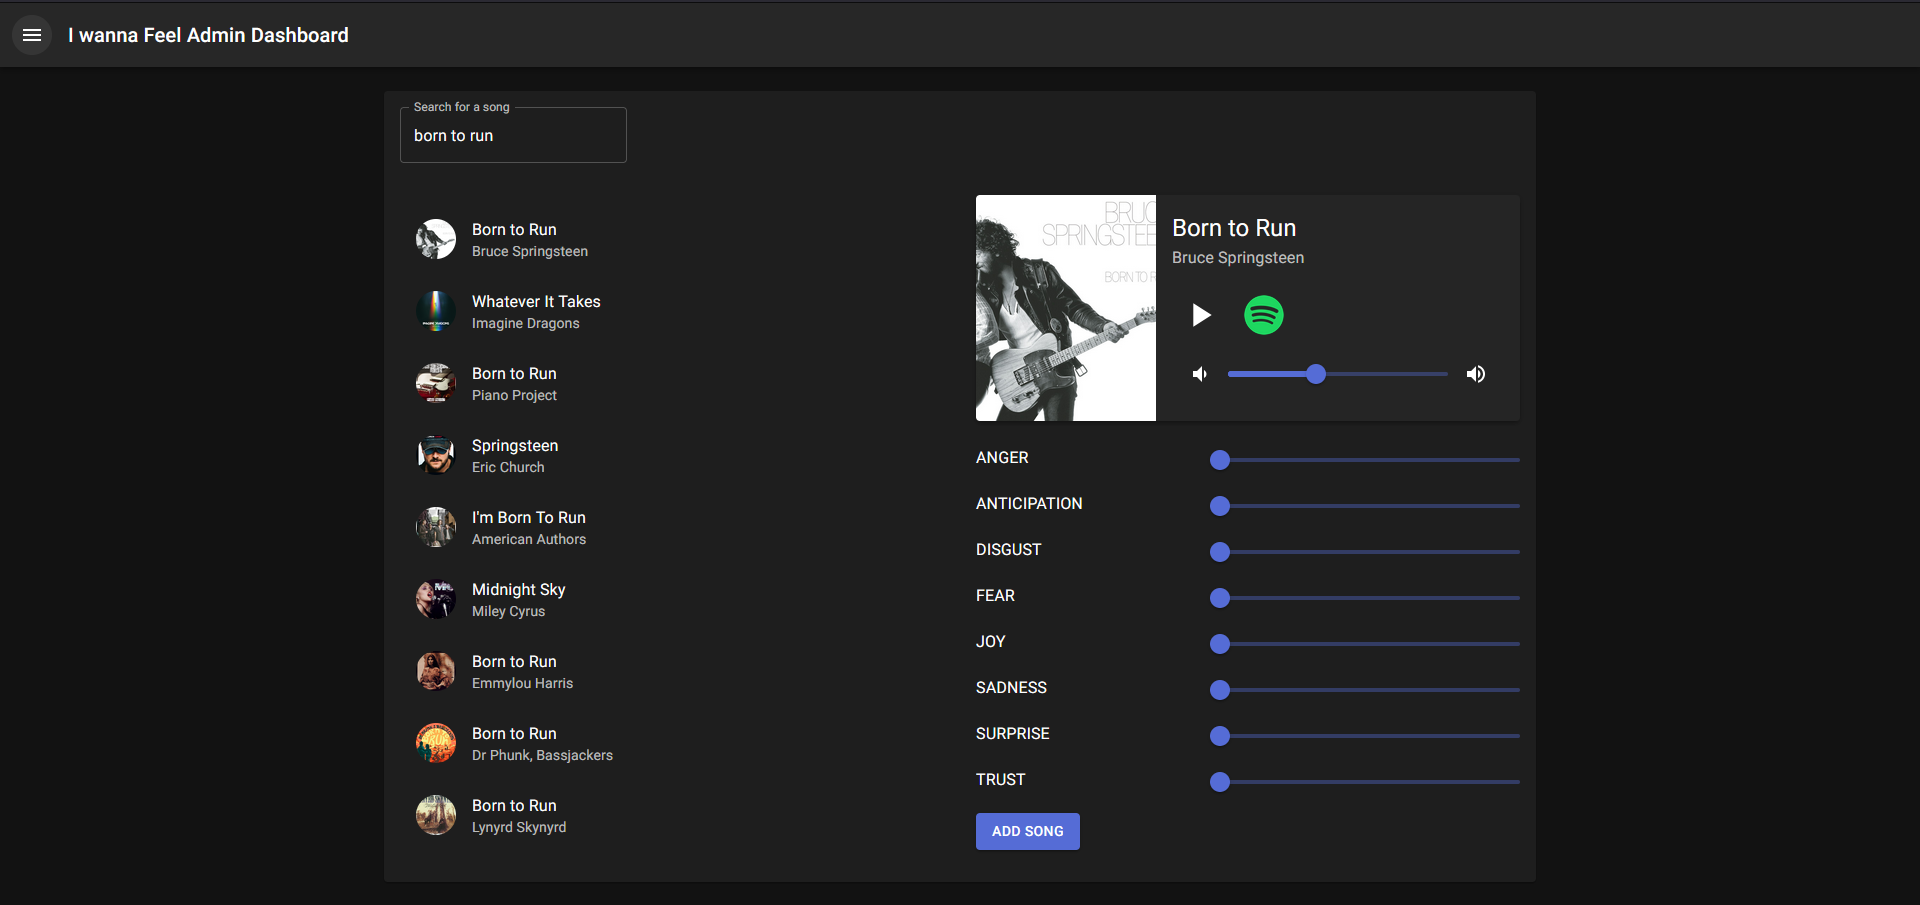
\includegraphics[width=\textwidth]{imgs/data_collection_1.png}
\caption{Section to search, play and label songs}
\label{fig: data_collection_1}
\end{figure}

\begin{figure}[H]
\centering
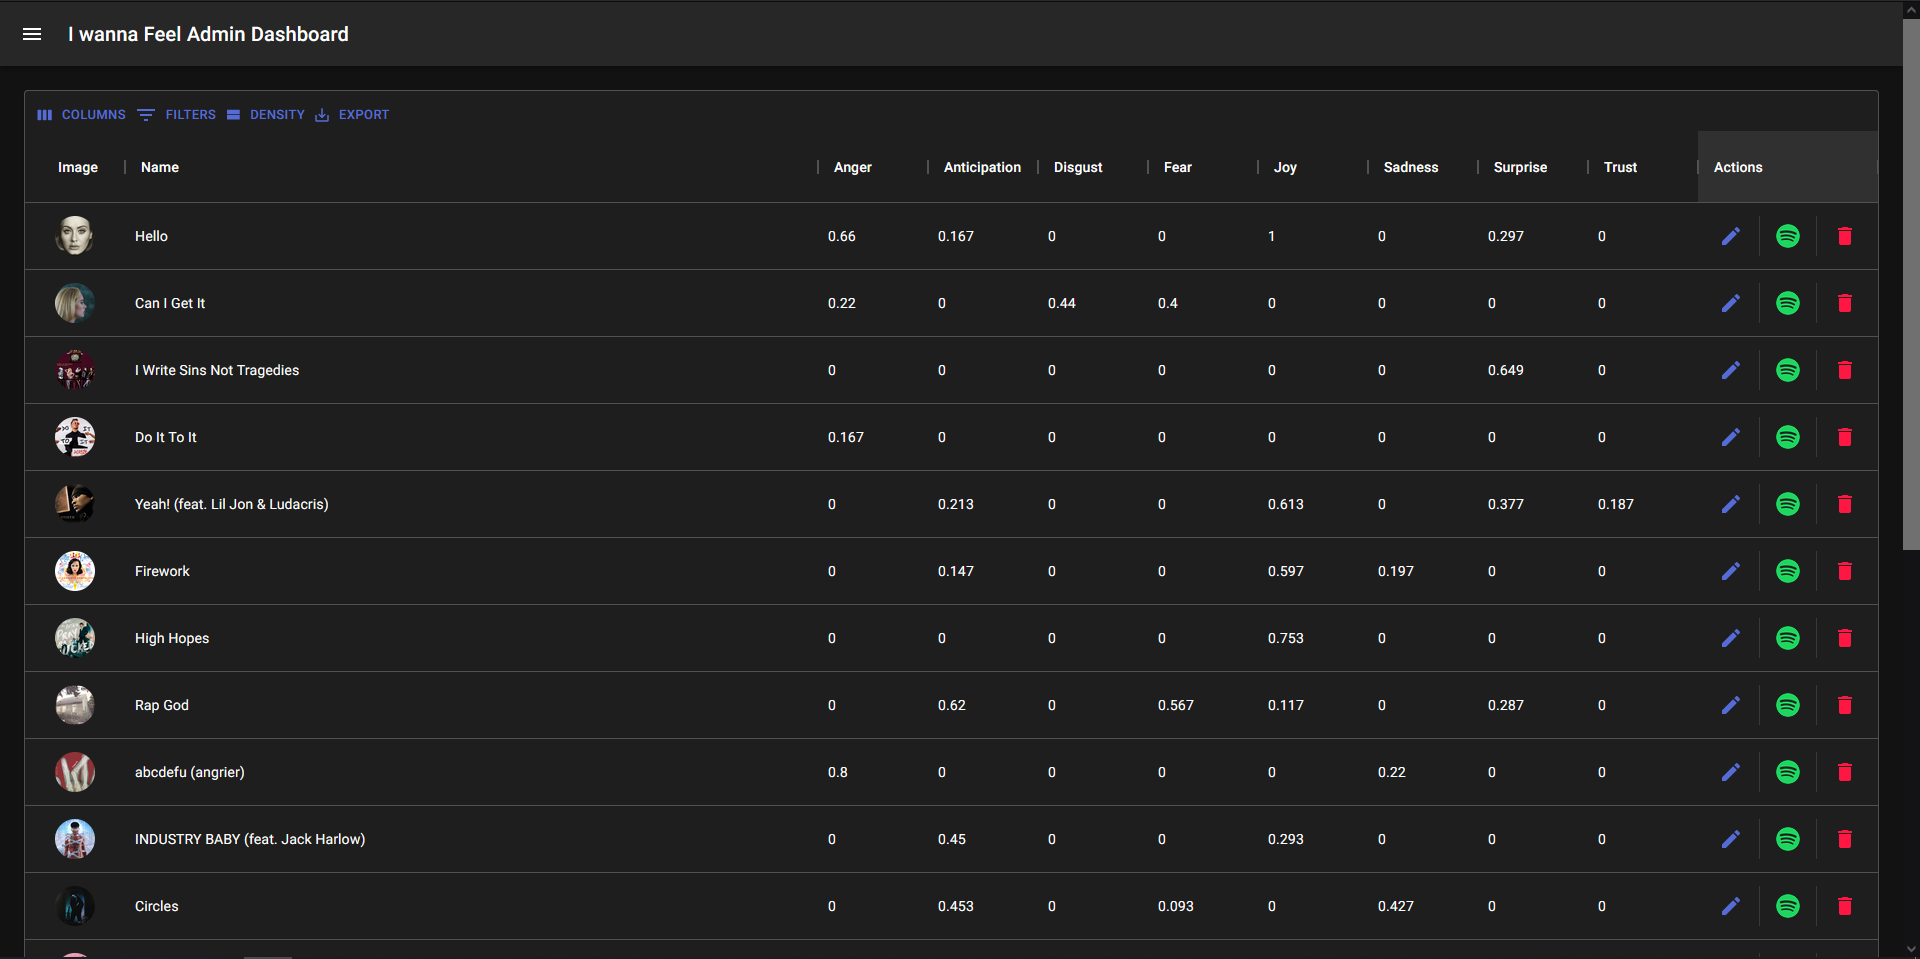
\includegraphics[width=\textwidth]{imgs/data_collection_2.png}
\caption{Section to search, filter, update, delete songs}
\label{fig: data_collection_2}
\end{figure}

\subsection{Mobile View}

\begin{figure}[H]
\centering
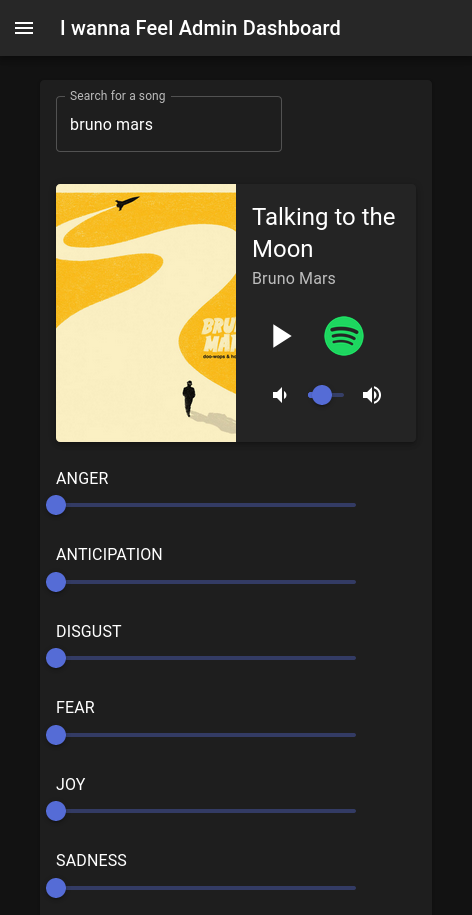
\includegraphics[scale=0.6]{imgs/mobileui1.png}
\caption{Emotion input}
\label{fig: mobileUI_1}
\end{figure}

\begin{figure}[H]
\centering
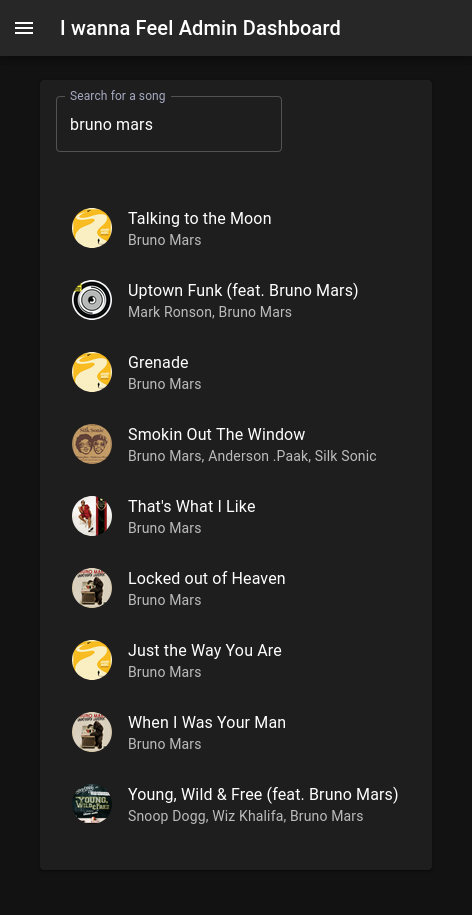
\includegraphics[scale=0.6]{imgs/mobileui2.png}
\caption{Song Search}
\label{fig: mobileUI_2}
\end{figure}

\begin{figure}[H]
\centering
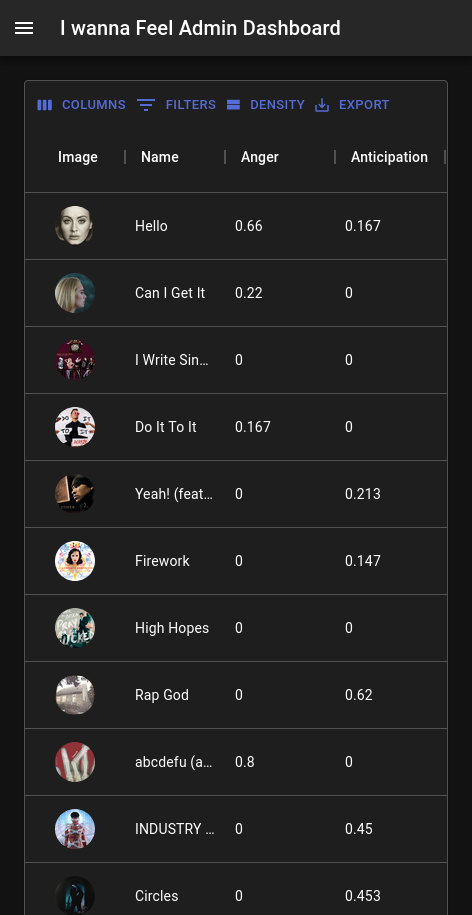
\includegraphics[scale=0.6]{imgs/mobileui3.png}
\caption{Database View}

\label{fig: mobileUI_3}
\end{figure}


\section{User Interface}
\subsection{Landing Page}
\begin{figure}[H]
\centering
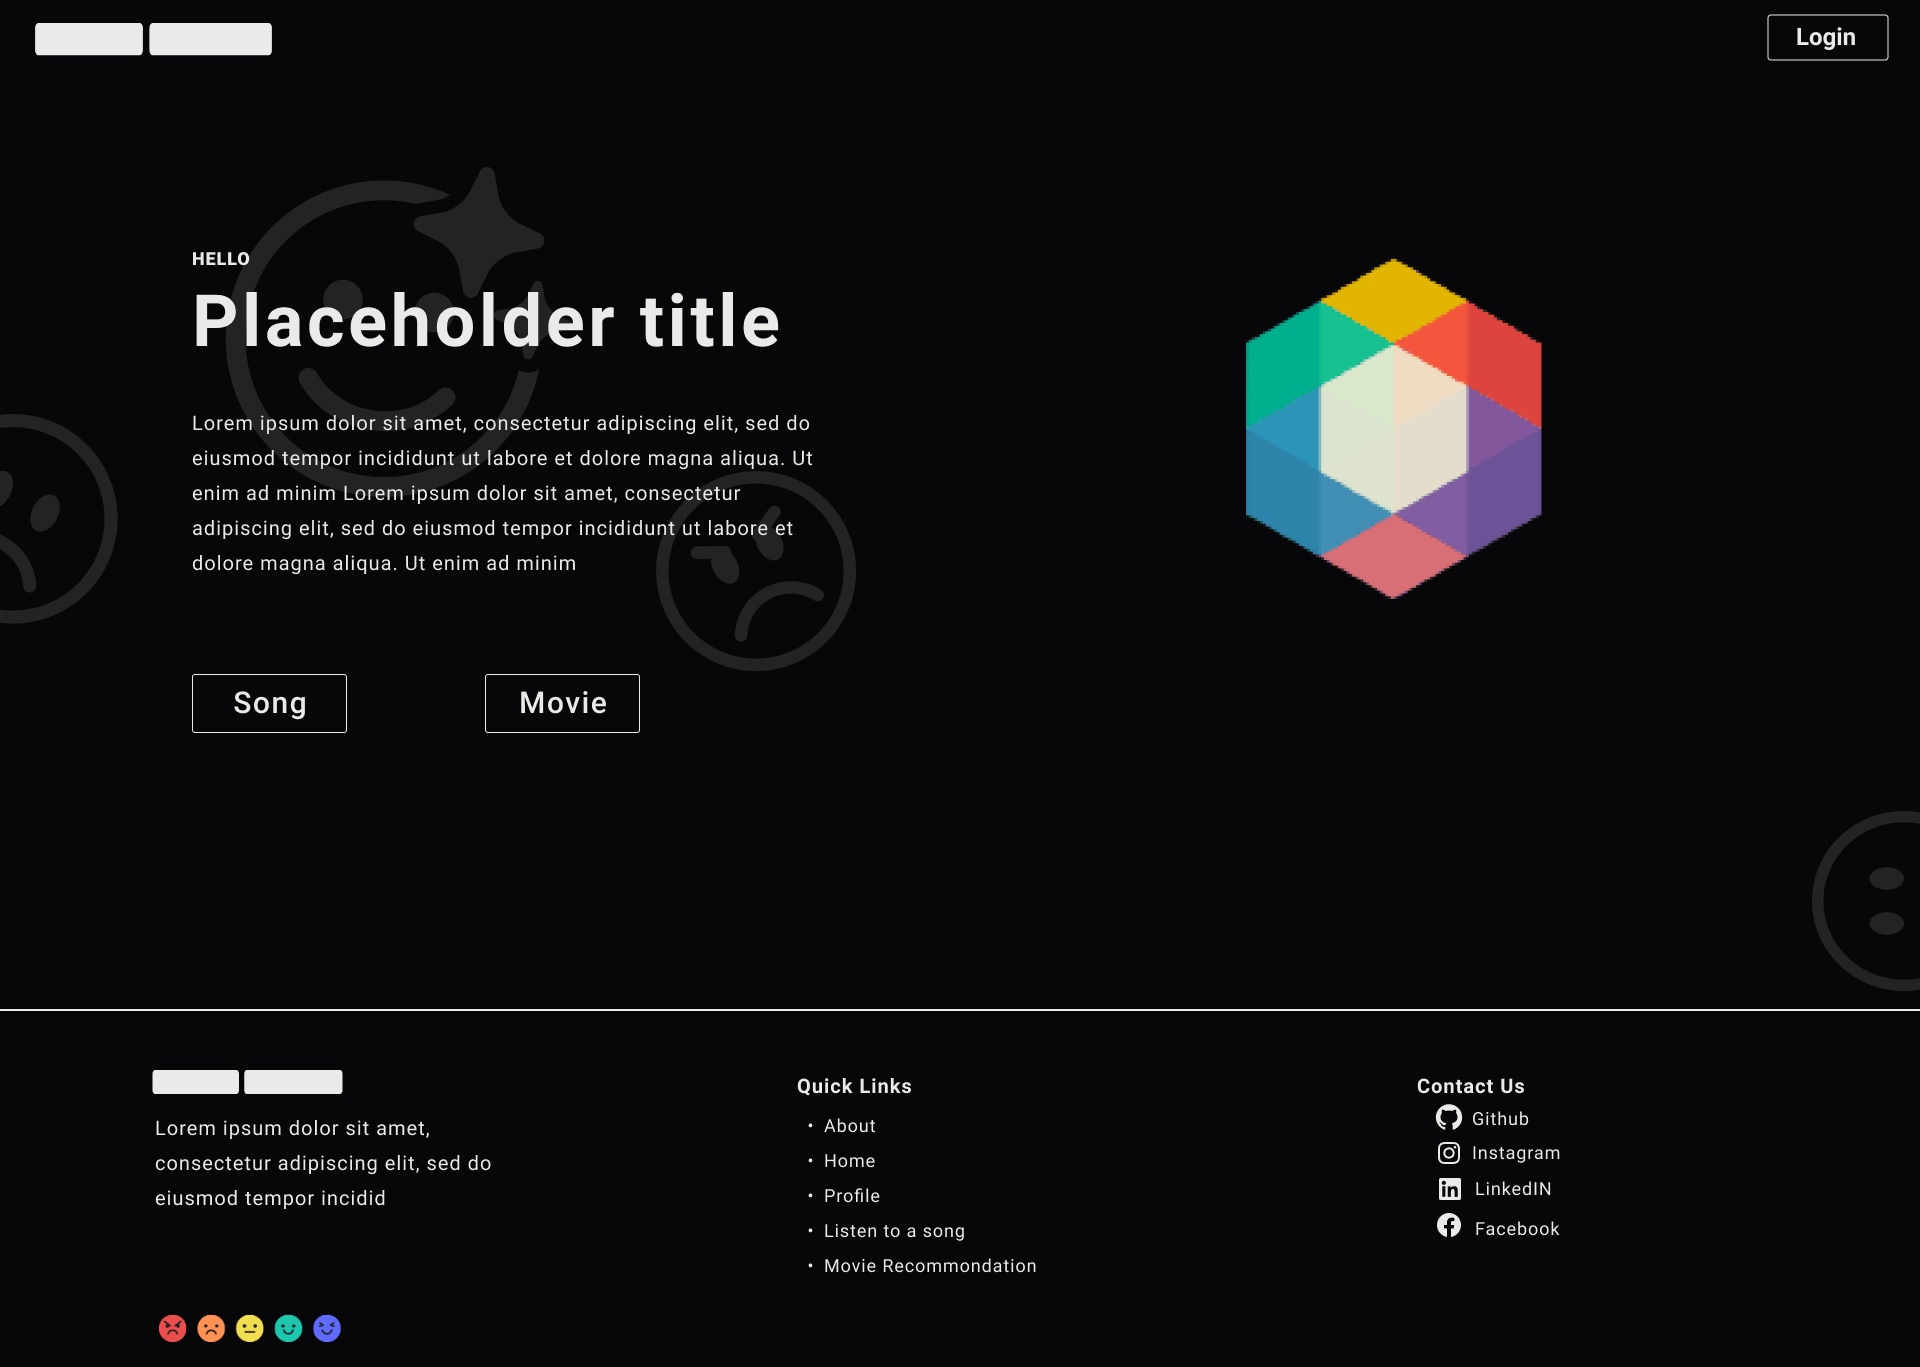
\includegraphics[width=\textwidth]{imgs/ui1.png}
\caption{Landing Page}
\label{fig: ui1}
\end{figure}

This is the home page, here there are 2 primary actions available which directs the user to the song search page or movie search page. The user can also choose to login from this page, but that is available on all pages as well.


\subsection{Emotion Input Pages}
\begin{figure}[H]
\centering
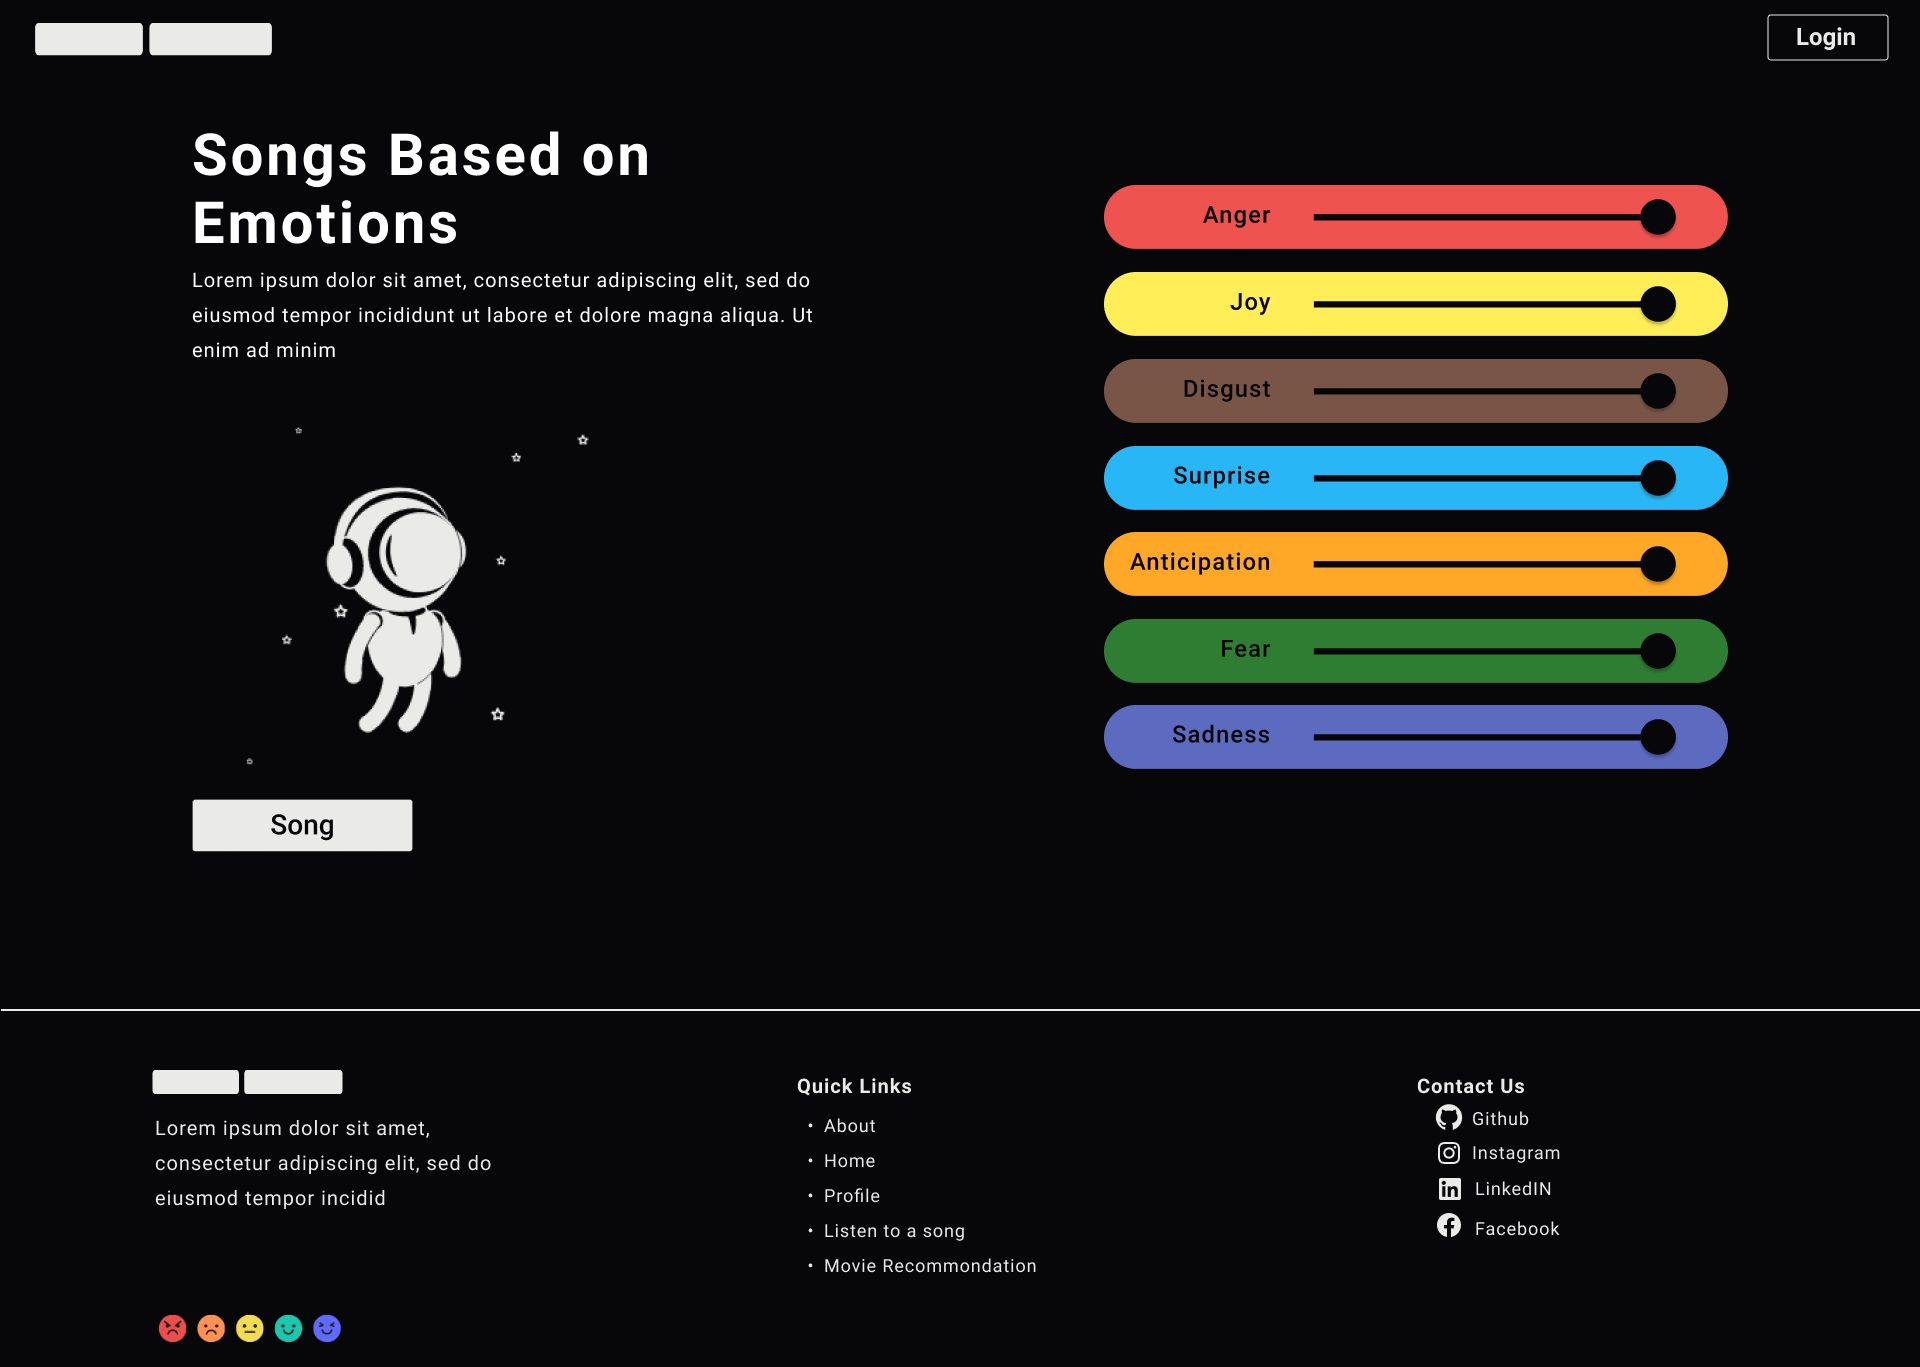
\includegraphics[width=\textwidth]{imgs/ui2.png}
\caption{Song Emotion Input Page}
\label{fig: ui2}
\end{figure}

\begin{figure}[H]
\centering
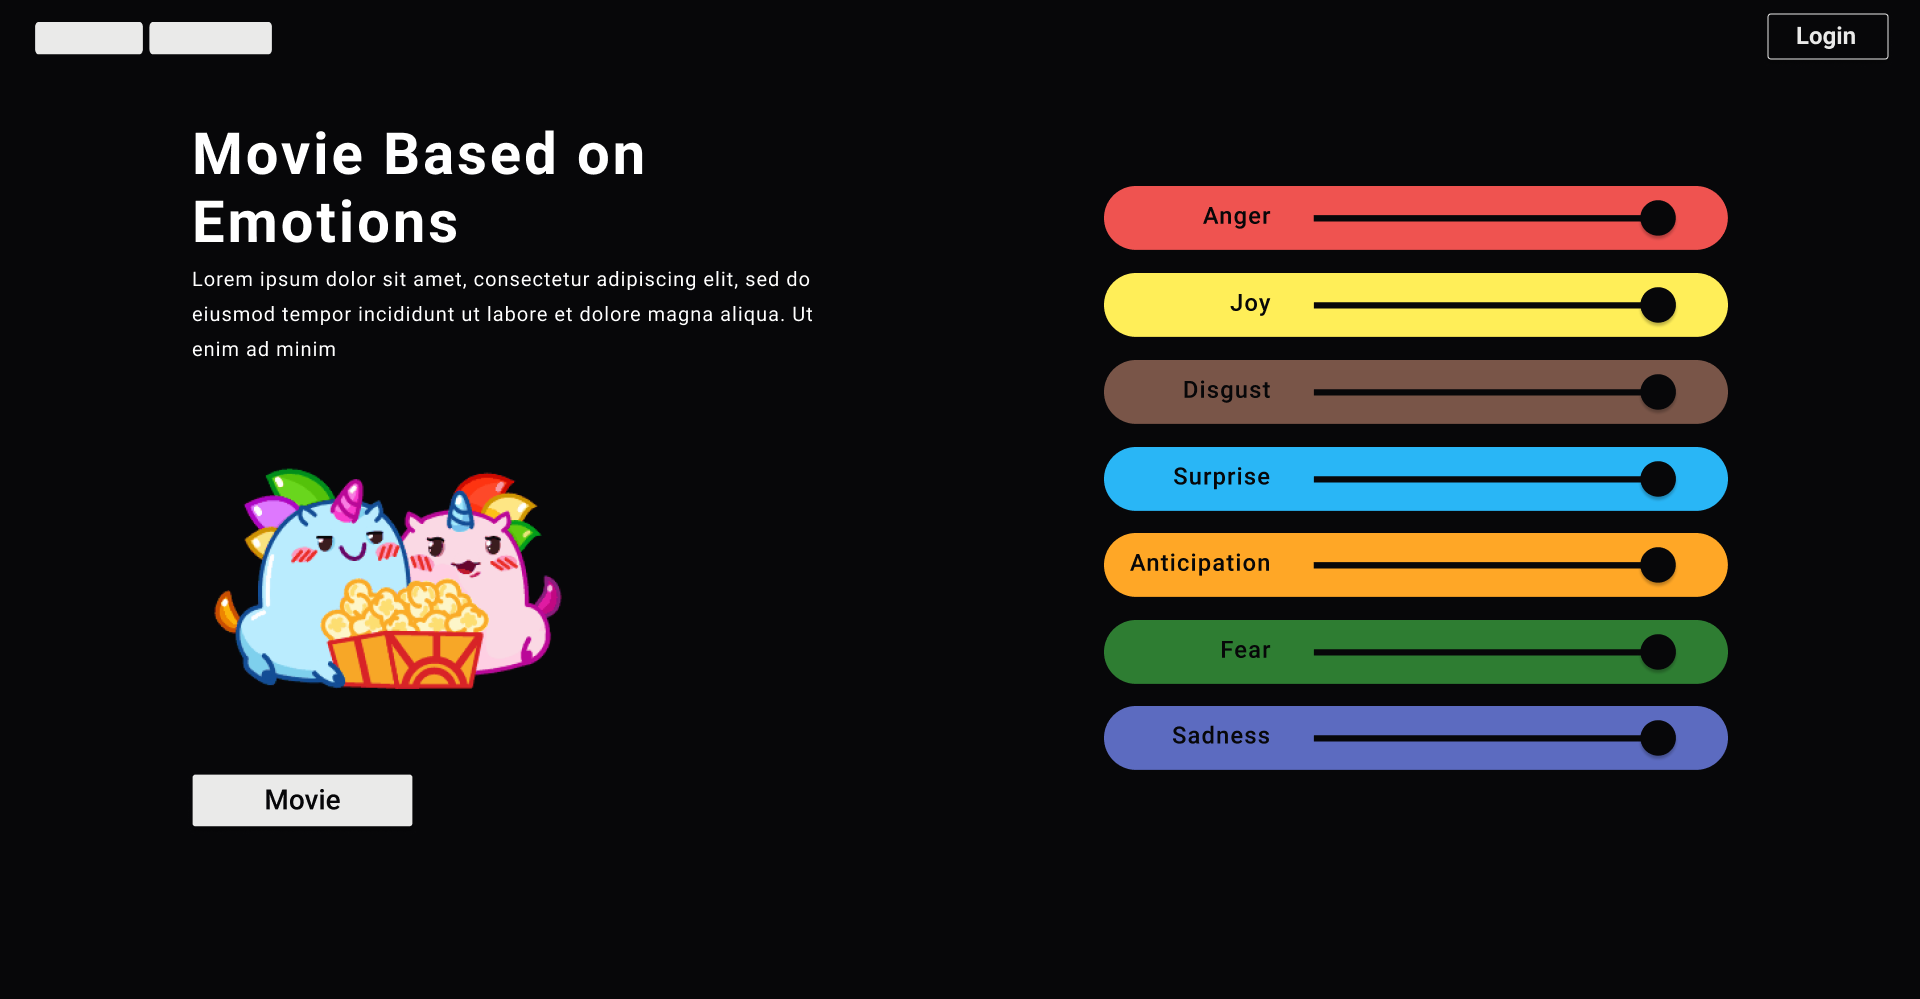
\includegraphics[width=\textwidth]{imgs/ui3.png}
\caption{Movie Emotion Input Page}
\label{fig: ui3}
\end{figure}

These are the emotion input pages, Figure \ref{fig: ui2} for songs and figure \ref{fig: ui3} for movies. Later, we plan to adjust the emotions for songs as we build our dataset. There are various sliders for the different available emotions.

\subsection{Recommendation Pages}
\begin{figure}[H]
\centering
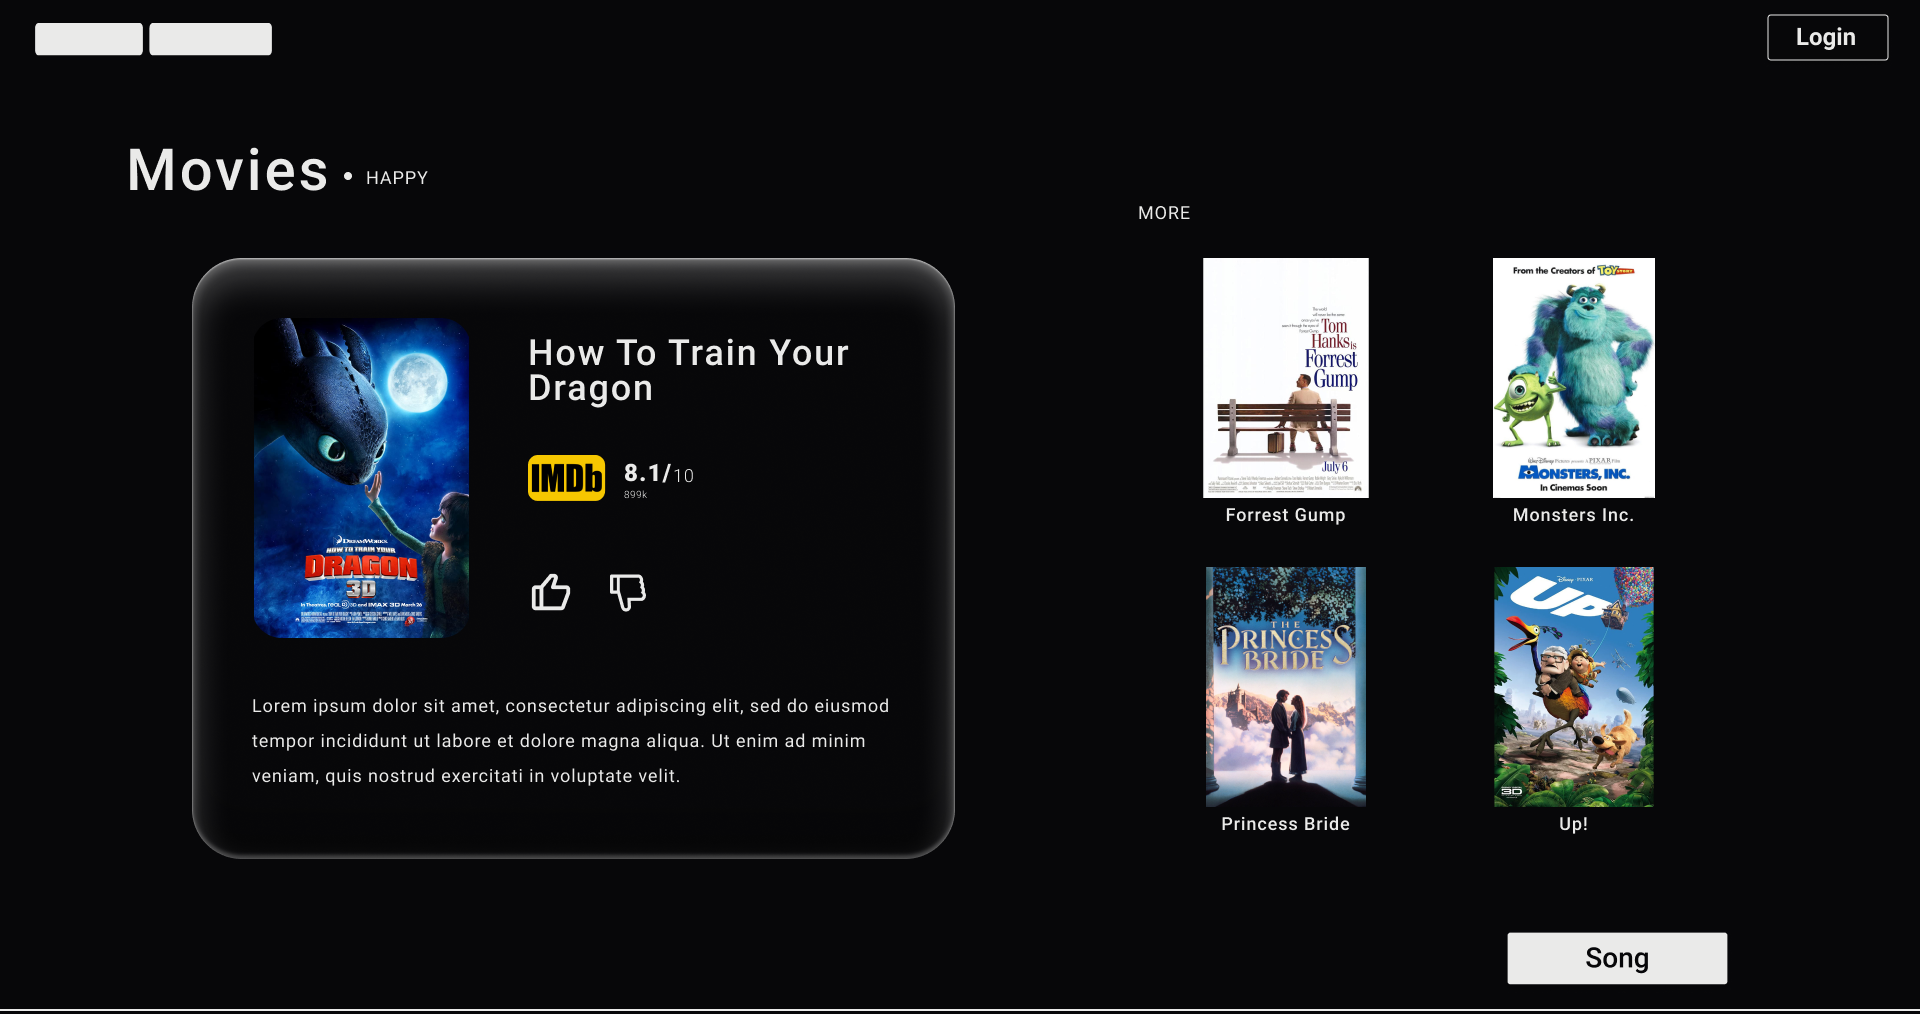
\includegraphics[width=\textwidth]{imgs/ui4.png}
\caption{Movie Suggestion Page}
\label{fig: ui4}
\end{figure}

\begin{figure}[H]
\centering
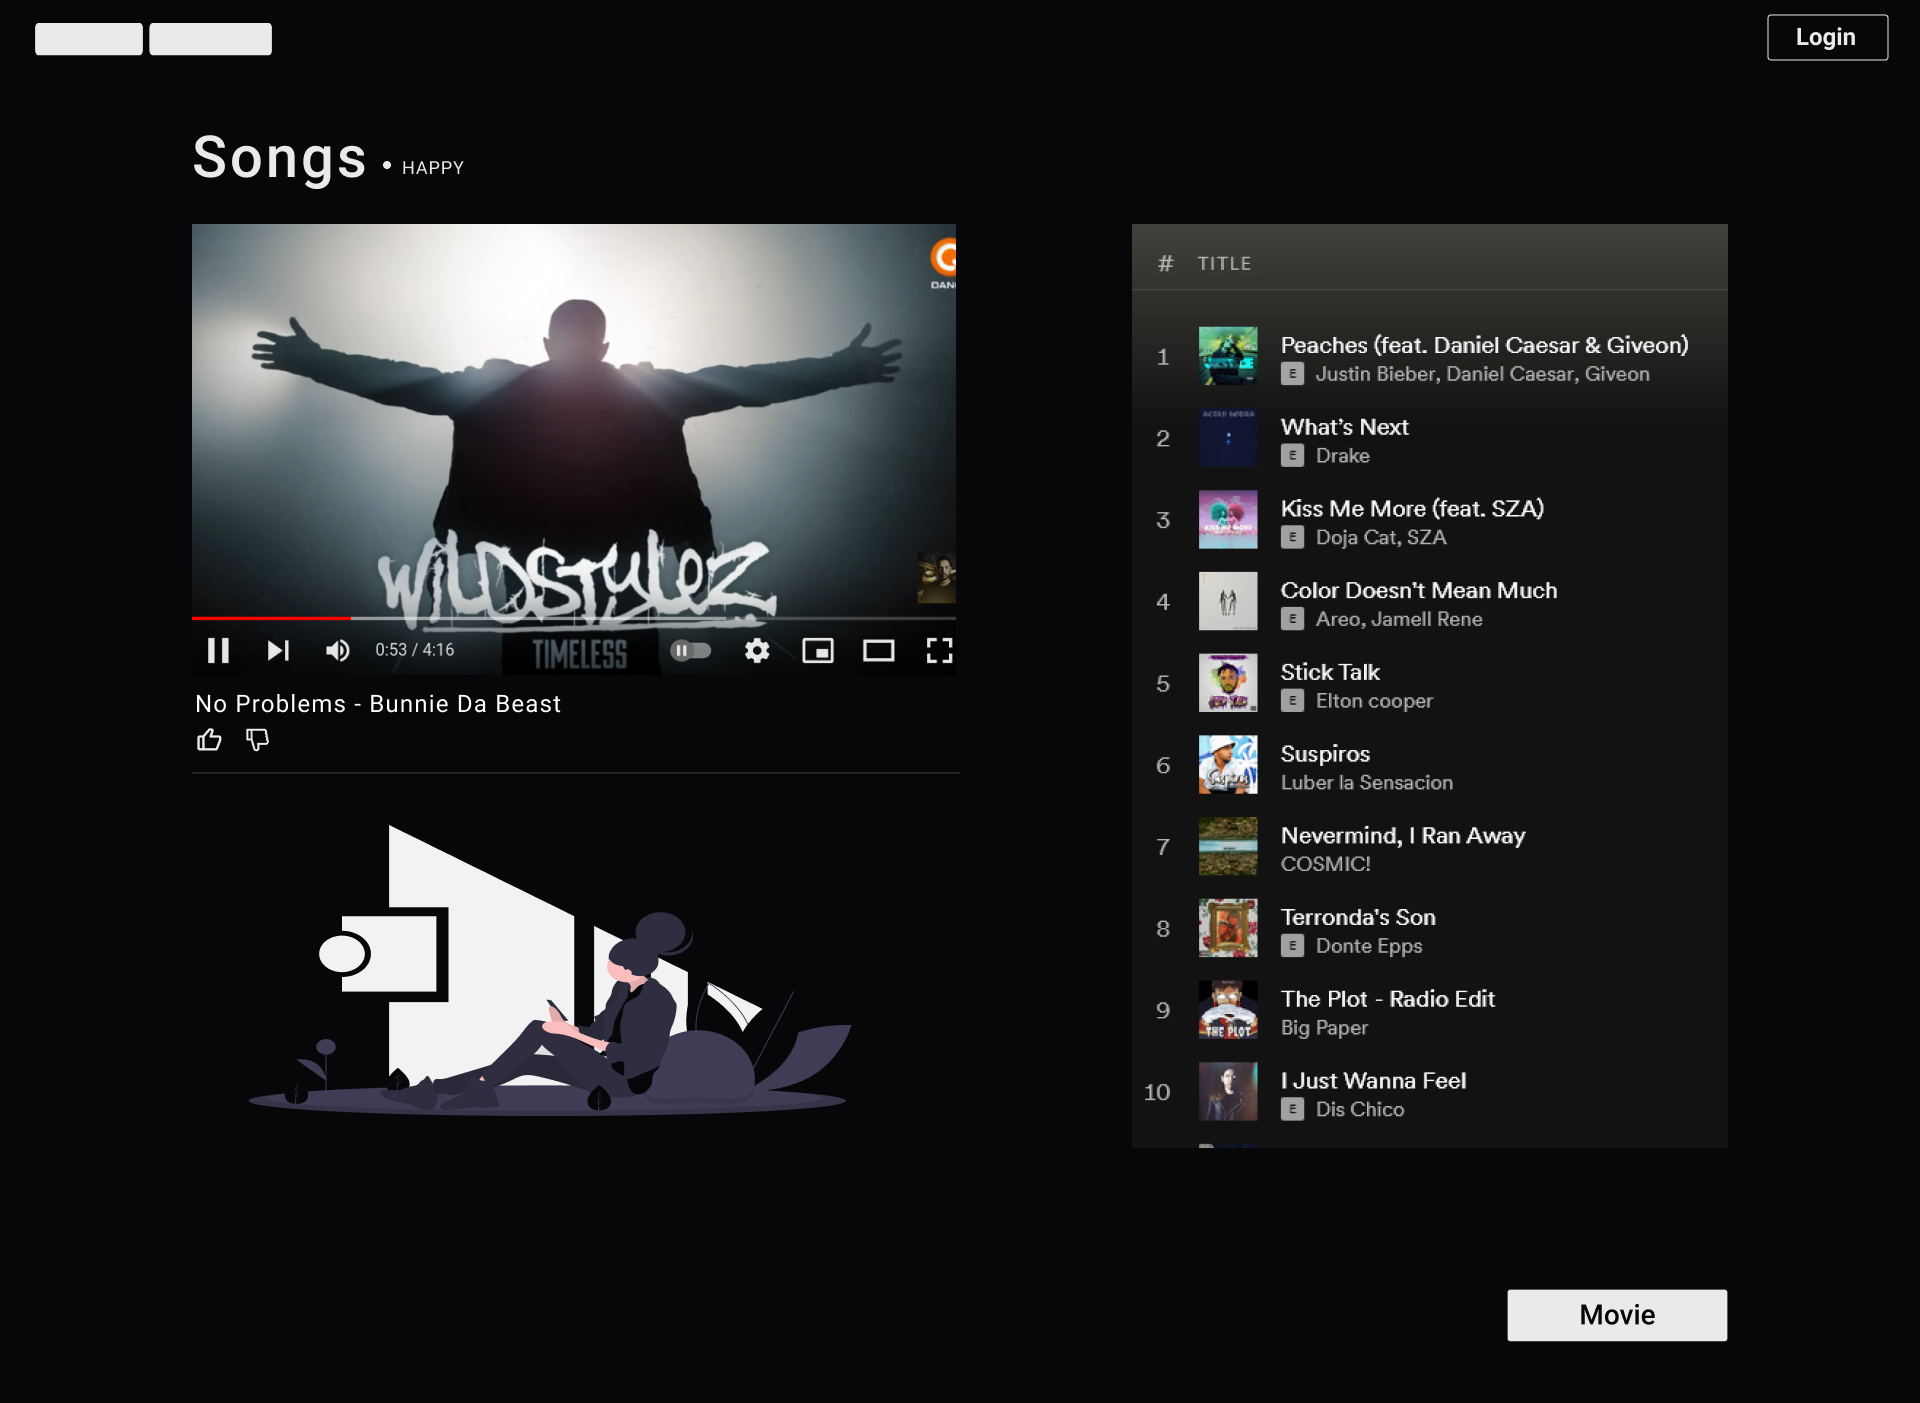
\includegraphics[width=\textwidth]{imgs/ui5.png}
\caption{Song Suggestion Page}
\label{fig: ui5}
\end{figure}
On these pages the user is recommended content based on the emotions inputted from the previous screen. The user is recommended the content in the form of a list, where they can click on it to see more info about it.For songs, we can show an embedded YouTube video. For movies, we can provide a link to IMDB / the content on an OTT platform like Amazon Prime / Netflix.

\subsection{Login Page}
\begin{figure}[H]
\centering
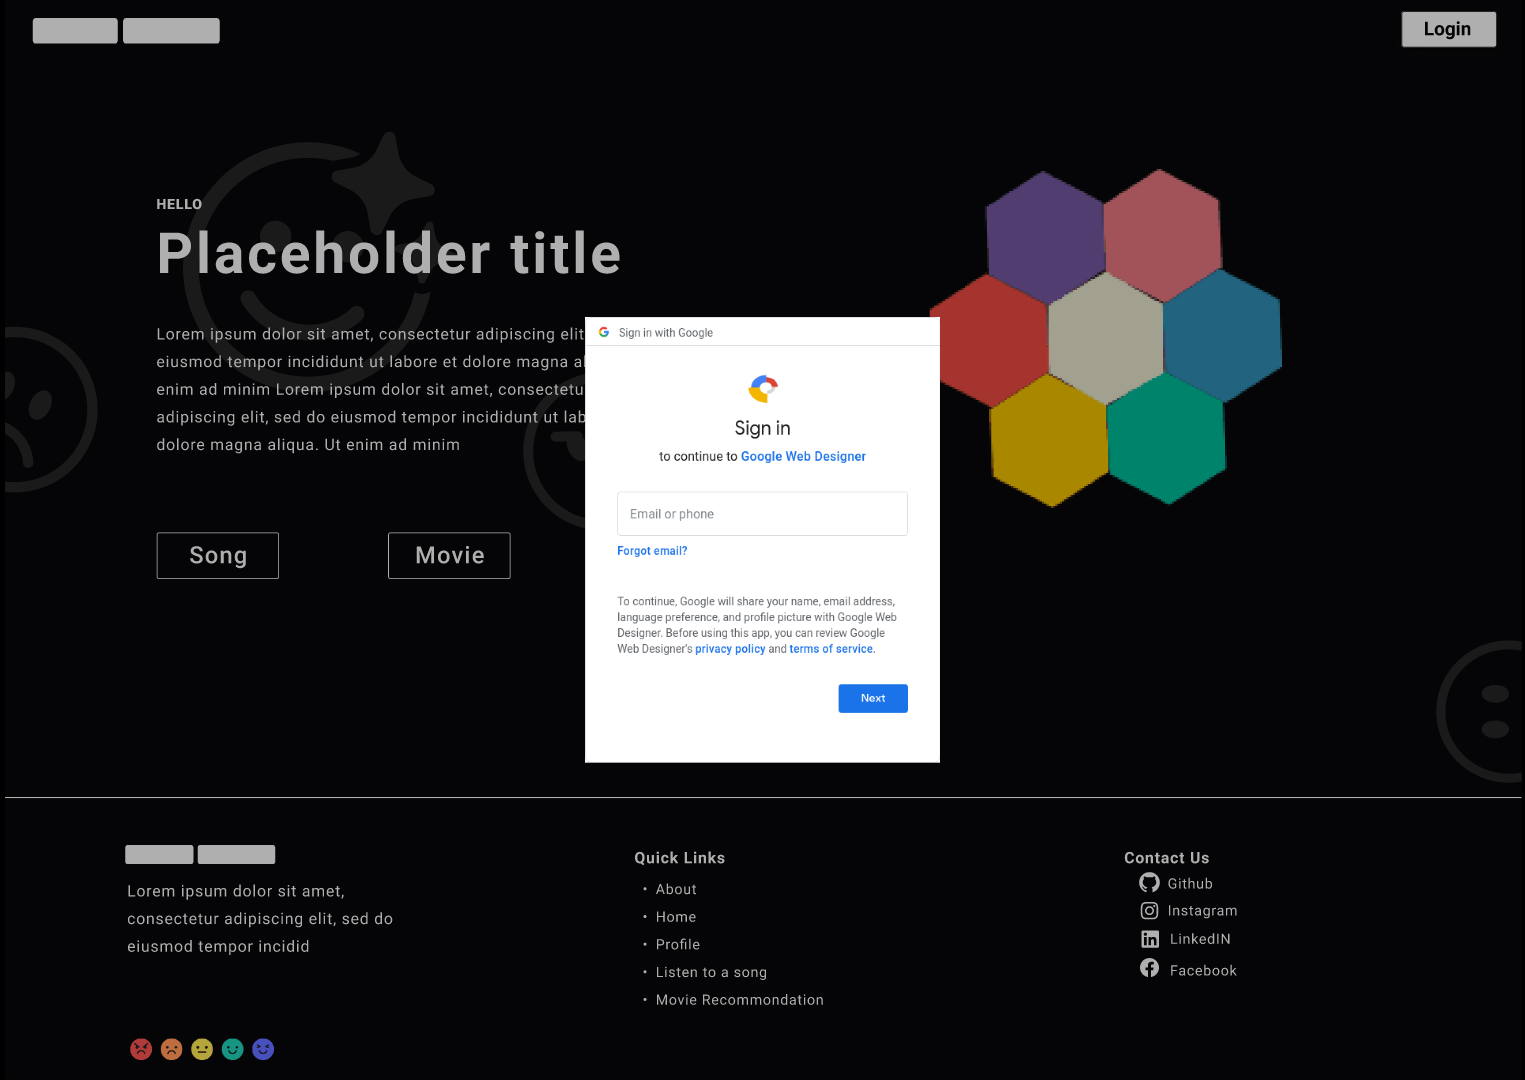
\includegraphics[width=\textwidth]{imgs/ui6.png}
\caption{Login Page}
\label{fig: ui6}
\end{figure}
The login will use Auth0 and will be available across all pages. It will appear as a popup and will provide a one-click login experience. The user will select from a list of services for authentication like Google, Github etc.





\chapter{Conclusion and Future Work}
\section{Conclusion}
%TODO
We have finished the literature survey, application design and UI design. \newline

The application we create will provide end users with a novel, transparent way of browsing and discovering new content.

\section{Future Work}
\begin{figure}[H]
\centering
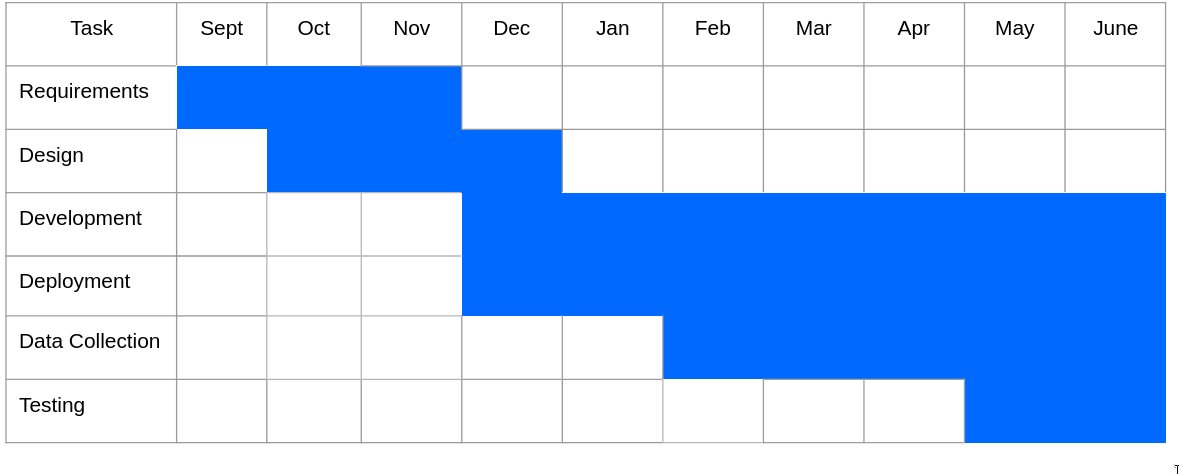
\includegraphics[width=\textwidth]{imgs/timeline.png}
\caption{Timeline}
\label{fig: timeline}
\end{figure}
Figure \ref{fig: timeline} shows the tentative project timeline. Beginning with requirements. We gathered information about what would be required to build the project between September and November. Our Design phase lasted till December.\newline
We are using a CI/CD mode of development so Development and Deployment is being done side by side. This way if there are any incompatibilities  that arise during deployment we can catch and fix them.\newline
In March we will begin data collection for the song recommender using the tool we showed you previously, once we collect around 200 data points we will begin developing the preprocessing pipelines and initial model tests. We will continue collecting data side by side with development as more data is always better.
We expect to have a minimum viable product by May, so we will begin testing at that point.


\printbibliography
\end{document}
